\documentclass[11pt,twocolumn,a4paper]{article}

\usepackage[utf8]{inputenc}
\usepackage[T1]{fontenc}
\usepackage{lmodern}
\usepackage[a4paper,margin=2.1cm,columnsep=0.55cm]{geometry}
\usepackage{amsmath,amssymb,amsthm,mathtools}
\usepackage{bm}
\usepackage{mathrsfs}
\usepackage{booktabs}
\usepackage{array}
\usepackage{enumitem}
\usepackage{microtype}
\usepackage{xcolor}
\usepackage{graphicx}
\usepackage{algorithm}
\usepackage{algpseudocode}
\usepackage[round,sort&compress]{natbib}
\usepackage[colorlinks=true,linkcolor=blue!45!black,
            citecolor=blue!45!black,urlcolor=blue!45!black]{hyperref}
\usepackage{cleveref}

\newtheoremstyle{rdm}{\topsep}{\topsep}{\itshape}{}{\bfseries}{.}{.5em}{}
\theoremstyle{rdm}
\newtheorem{theorem}{Theorem}[section]
\newtheorem{lemma}[theorem]{Lemma}
\newtheorem{proposition}[theorem]{Proposition}
\newtheorem{corollary}[theorem]{Corollary}
\theoremstyle{definition}
\newtheorem{definition}[theorem]{Definition}
\newtheorem{axiom}{Axiom}
\newtheorem{construction}[theorem]{Construction}
\newtheorem{example}[theorem]{Example}
\theoremstyle{remark}
\newtheorem{remark}[theorem]{Remark}

% ---------------------------------------------------------------------
% Notation shared with, and consistent across, the source manuscripts.
% ---------------------------------------------------------------------
\newcommand{\Cands}{X}
\newcommand{\Know}{K}
\newcommand{\Om}{\Omega}
\newcommand{\flo}{\mathrm{flo}}
\newcommand{\Rec}{R}
\newcommand{\Fed}{\mathcal{F}}
\newcommand{\dem}{D}
\newcommand{\str}{\sigma}
\newcommand{\rg}{\mathfrak{r}}
\newcommand{\Cat}{\mathrm{Cat}}
\newcommand{\reach}{\mathrm{Reach}}
\newcommand{\argmax}{\operatorname*{arg\,max}}

\title{\textbf{The Distributed Domain Route Graph: Routing, Water-Filling,
and Phase-Locked Federation for a Population of Opaque Domain Receivers}}
\author{Kundai Farai Sachikonye}
\date{}

\begin{document}
\maketitle

\begin{abstract}
\emph{Accountable Compilation} \citep{sachikonye-accountable-compilation}
shows that any \emph{given} finite collection of bounded receivers composes
under federation, cascade allocation, and cross-verification with a
provable, non-zero floor. It does not say which receivers to consult, nor
what to do when the receivers consulted number more than a handful and must
be combined \emph{live}, at query time, rather than composed once, offline,
into a fixed architecture, nor — most fundamentally — how much agreement
between two receivers is \emph{sufficient} to certify a lock, as opposed to
a hand-chosen tolerance. Three independent manuscripts by the same author
supply, without citing one another or the receiver formalism directly,
the missing pieces: \emph{Federated Context Closure}
\citep{sachikonye-federated-context-closure} shows that a router can be
built to record only the \emph{shape} of what closed a question, never the
content that closed it, so that a central coordinator never needs the
private material of whatever it routes to; \emph{Split-Attention
Synchronised Agents} \citep{sachikonye-split-attention} shows that a bounded
capacity budget divided by water-filling across concurrently-consulted
agents, and a population of such agents driven toward Kuramoto phase-lock
\citep{kuramoto1975}, both obey closed-form laws with an exact optimum and a
provable synchronisation threshold; and \emph{Coordination Regimes of
Synchronised Agents} \citep{sachikonye-coordination-regimes} shows that the
stopping criterion for agreement is not a graded residual at all but a
\emph{binary} categorical-distinguishability condition — partition
extinction — whose transition is provably discontinuous, replacing a
tunable tolerance with a quantity derived from the model's own finite
resolution. This paper proves that these results compose: that a route
graph is itself a bounded receiver in the sense of
\citet{sachikonye-accountable-compilation}, that water-filling is the
continuous relaxation of the Cascade Theorem's discrete knapsack as the
number of consulted receivers grows, that a federation of
extinction-locked, individually-opaque receivers inherits a floor that
sharpens geometrically in the number of \emph{locked} members while
\emph{necessarily} — not merely by design choice — excluding, rather than
averaging in, members that fail to lock, that this exclusion is licensed by
an observable-commutation result separating functional lock from internal
opacity, and that the whole assembly is again a bounded receiver — closing
the loop, so that a federation of federations is not a new kind of object.
Eight computational experiments validate each composed claim against exact
or simulated ground truth.
\end{abstract}

% =====================================================================
\part{The Problem Accountable Compilation Leaves Open}
\label{part:problem}
% =====================================================================

\section{Introduction}
\label{sec:intro}

Consider a population of $N$ independently-trained, independently-owned
domain receivers $\Rec_1,\dots,\Rec_N$ — in the terms of
\citet{sachikonye-accountable-compilation}, each a bounded receiver
(\Cref{def:receiver-recap}) acquired once, at its own domain's extremal
regime, by that paper's acquisition pipeline. A central coordinator, itself
a receiver, must answer a query $x$ using this population without ever
holding, training on, or decoding any member's internal knowledge state
$\Know_i$ — the coordinator and every $\Rec_i$ form an opaque pair
(\Cref{def:opaque-recap}) for every $i$, pairwise. \emph{Accountable
Compilation}'s Federation, Cascade, and Verification-Floor theorems govern
what happens once a subset of the population, and a budget for consulting
it, are already fixed: the joint floor of a chosen federation is bounded
(\Cref{thm:federation-recap}), the value-optimal subset under a hard budget
is a solvable knapsack (\Cref{thm:cascade-recap}), and a verification step
between two opaque receivers is itself a receiver with its own composable
floor (\Cref{thm:verif-floor-recap}). None of these results addresses three
questions that arise the moment $N$ is large and the population is queried
live rather than composed once offline:

\begin{enumerate}[nosep]
\item \textbf{Selection.} \emph{Which} receivers, out of $N$ that the
coordinator has never inspected, are worth consulting for a given query,
without the coordinator ever having seen their content?
\item \textbf{Allocation.} Given a fixed total query budget and more
candidate receivers than the budget can fully afford, how should the budget
be \emph{divided} — not merely which $0/1$ subset to admit, but how much
attention or compute each admitted receiver receives?
\item \textbf{Combination.} Once several receivers respond concurrently,
how are their responses combined into one certified output, in a way that
correctly \emph{declines} to include a receiver whose response is out of
step with the rest, rather than silently averaging an outlier in?
\end{enumerate}

\Cref{sec:closure} answers Selection by showing a \emph{route graph}
recording only closure-shape, not content, is itself a bounded receiver.
\Cref{sec:waterfill} answers Allocation by showing water-filling is the
continuous limit of the Cascade Theorem's discrete knapsack.
\Cref{sec:phaselock} answers Combination by proving a phase-locked
federation's floor sharpens geometrically in the number of \emph{locked}
members and by making the exclusion of unlocked members precise;
\Cref{sec:extinction} then sharpens Combination's own stopping criterion,
replacing the hand-set lock tolerance with a derived, binary one and
showing the exclusion of unlocked members is forced rather than chosen.
Sections \ref{sec:elimination} and~\ref{sec:seam} close the loop: a
receiver in this
population is required to expose only a negation set, never a decoded
value, and the whole three-layer assembly — route, allocate, combine — is
itself a bounded receiver, so a federation of federations is governed by
exactly the same laws as a federation of leaves.

\section{Preliminaries: A Shared Notation for Three Independent
Formalisms}
\label{sec:prelim}

The three source manuscripts state structurally identical objects under
different names, having been derived independently rather than by one
building on another. \Cref{tab:notation} fixes one notation for this paper;
all subsequent statements use the right-hand column.

\begin{table}[!htbp]
\centering
\small
\begin{tabular}{@{}p{0.20\linewidth}p{0.20\linewidth}p{0.20\linewidth}p{0.20\linewidth}@{}}
\toprule
\textbf{Object} & \citet{sachikonye-accountable-compilation} & \citet{sachikonye-federated-context-closure} & This paper \\
\midrule
Worst-case residual & $\flo(\Rec)$ & floor $\beta$ (three independent derivations) & $\flo(\Rec)$ \\
Bounded agent & receiver $\Rec=(\Know,\Phi,\Pi)$ & --- (asker/context $\Gamma_u$) & receiver $\Rec$ \\
Never-decoded pairing & opaque pair (\Cref{def:opaque-recap}) & --- & opaque pair \\
Evidence unit & column $a=\Pi(\Phi(x))$ & catalyst $\Cat=(\mathrm{src},\rho_{\Cat})$ & column / catalyst (used interchangeably; \Cref{def:catalyst-as-column}) \\
Termination criterion & quiescence (\Cref{def:quiescence-recap}) & closure (reach-set equality) & quiescence (\Cref{def:quiescence-recap}, reused for route-graph termination in \Cref{def:route-receiver}) \\
\bottomrule
\end{tabular}
\caption{Three independent papers' names for structurally identical
objects. \citet{sachikonye-split-attention} is omitted from the table
because it introduces genuinely new objects (a capacity budget, a phase)
rather than a renamed floor/receiver pair; its notation is introduced fresh
in \Cref{sec:waterfill,sec:phaselock}.}
\label{tab:notation}
\end{table}

We restate, without reproof, the four prior results this paper builds on.

\begin{definition}[Receiver, restated]
\label{def:receiver-recap}
A \emph{receiver} on outcome space $(\Cands,d,\Om)$ is
$\Rec=(\Know,\Phi,\Pi)$ with $\Know$ finite, $\Phi:\Cands\to\Know$, and
$\Pi:\Know\to 2^{\Cands}\setminus\{\varnothing\}$ satisfying
$\Phi(x)\in\Phi(\Pi(\Phi(x)))$; its floor is
$\flo(\Rec)=\sup_x\inf_{x'\in\Pi(\Phi(x))}d(x,x')$, strictly positive
whenever $|\Know|<|\Cands|$
\citep[Def.~5.2, Thm.~5.1]{sachikonye-accountable-compilation}.
\end{definition}

\begin{definition}[Opaque pair, restated]
\label{def:opaque-recap}
$\Rec_A,\Rec_B$ are an \emph{opaque pair} if no computable
$h:\Know_A\to\Know_B$ (or conversely) satisfies $\Phi_B=h\circ\Phi_A$ on
their common domain
\citep[Def.~8.1]{sachikonye-accountable-compilation}.
\end{definition}

\begin{definition}[Quiescence and decline, restated]
\label{def:quiescence-recap}
\label{def:decline-recap}
The four-column relaxation between an opaque pair is \emph{quiescent} at
round $r^\star$ if the joint residual $\dem^{(r^\star)}$ (central plus
provoked residuals of \citet[Def.~8.3]{sachikonye-accountable-compilation})
falls below tolerance $\tau=\flo(\Rec_A)+\flo(\Rec_B)$ and does not
subsequently exceed it; otherwise the pair \emph{declines}, reporting
non-quiescence rather than an arbitrarily chosen one of the two central
columns \citep[Def.~8.4, Thm.~8.2]{sachikonye-accountable-compilation}.
\end{definition}

\begin{theorem}[Quiescence certifies agreement without disclosure, restated]
\label{thm:quiescence-formal-recap}
If the relaxation reaches quiescence, the pair's answers are
indistinguishable up to $\tau$ by any test computable from the four columns
alone, using no decoding map of the kind \Cref{def:opaque-recap} excludes
\citep[Thm.~8.1]{sachikonye-accountable-compilation}.
\end{theorem}

\begin{theorem}[Route-Audit, restated]
\label{thm:route-audit-recap}
\label{thm:route-audit}
There exist opaque pairs and queries for which the central residuals are
both below tolerance while the provoked residuals are not, so the pair is
non-quiescent although a central-columns-only comparison would report
agreement \citep[Thm.~8.3]{sachikonye-accountable-compilation}.
\end{theorem}

\begin{theorem}[Federation, restated]
\label{thm:federation-recap}
For a union-form federation $\Fed=\{\Rec_i\}_{i=1}^n$,
$\flo(\Fed)\le\min_i\flo(\Rec_i)$
\citep[Thm.~6.2]{sachikonye-accountable-compilation}.
\end{theorem}

\begin{theorem}[Multiplicative composition law, restated]
\label{thm:mult-law-recap}
If the receivers' resolution failures are independent in the sense that
``$\Pi_i(\Phi_i(x))$ fails to contain a point within $\eps$ of $x$'' is
independent across $i$ for every $x,\eps$, then
$1-\flo(\Fed)/\Om=\prod_i(1-\flo(\Rec_i)/\Om)$
\citep[Thm.~6.3]{sachikonye-accountable-compilation}.
\end{theorem}

\begin{theorem}[Cascade, restated]
\label{thm:cascade-recap}
Under budget $B$ and per-receiver cost $c_i$, the floor-minimising $0/1$
selection is the knapsack
$\alpha^\star=\argmax_\alpha\sum_i\alpha_i v_i$ s.t.\
$\sum_i\alpha_ic_i\le B$, $v_i=\log(\Om/(\Om-\flo(\Rec_i)))$, exact in
$O(kB)$ by dynamic programming and within $(1-1/e)$ of optimal by
value-density greedy
\citep[Thm.~6.4]{sachikonye-accountable-compilation}.
\end{theorem}

\begin{theorem}[Verification-Floor, restated]
\label{thm:verif-floor-recap}
The four-column relaxation between an opaque pair $\Rec_A,\Rec_B$ is itself
a receiver $\Rec_{AB}$ satisfying \Cref{def:receiver-recap}, with
$\flo(\Rec_{AB})\le\flo(\Rec_A)+\flo(\Rec_B)+\eta_{AB}$, $\eta_{AB}$ the
measure of queries on which the pair declines rather than reaching
quiescence, and $\Rec_{AB}$ is exempt from no further instance of the same
construction
\citep[Def.~9.1, Prop.~9.1, Thm.~9.1, Cor.~9.1]{sachikonye-accountable-compilation}.
\end{theorem}

% =====================================================================
\part{Selection: The Route Graph as a Receiver}
\label{part:selection}
% =====================================================================

\section{The Route Graph Never Holds Content}
\label{sec:closure}

\citet{sachikonye-federated-context-closure} defines a \emph{catalyst}
$\Cat=(\mathrm{src}(\Cat),\rho_\Cat)$ — a provenance label and a partial
function from queries to answer-regions — and a shared \emph{route graph}
$\rg$ recording, for each closed question-shape, \emph{which} catalyst
closed it, never the catalyst's content. Two theorems of that paper are
load-bearing here: closure is invariant to which source supplied a catalyst
(blindness) and to whether the catalyst is true (truth-blindness)
\citep[Thm.~4.2, 4.3]{sachikonye-federated-context-closure}. We now show the
route graph, read as an object querying a population of receivers, is
itself a receiver.

\begin{definition}[Catalyst as column]
\label{def:catalyst-as-column}
For a query $x$ and a receiver $\Rec_i$ with column $a_i=\Pi_i(\Phi_i(x))$,
the induced catalyst is $\Cat_i:=(\,i,\;x'\mapsto a_i\,)$ — the receiver's
own identity as provenance and its column as the (constant, at this query)
reach function. This identifies \citet{sachikonye-accountable-compilation}'s
column with \citet{sachikonye-federated-context-closure}'s catalyst exactly
at the level the route graph consumes: the route graph never inspects $a_i$
itself, only whether the catalyst $\Cat_i$ closed the query, matching Row~4
of \Cref{tab:notation}.
\end{definition}

\begin{definition}[Route-graph receiver]
\label{def:route-receiver}
Given a population $\{\Rec_i\}_{i=1}^N$ and a reference query distribution,
the \emph{route-graph receiver} $\Rec_\rg=(\Know_\rg,\Phi_\rg,\Pi_\rg)$ has
knowledge framework $\Know_\rg$ the finite set of observed
\emph{closure-shapes} (which subset of provenances closed a question of a
given syntactic type, in the sense of
\citet[Def.~4.2]{sachikonye-federated-context-closure}); decoder
$\Phi_\rg(x)$ the closure-shape actually observed for $x$; and candidate
projection $\Pi_\rg(\Phi_\rg(x))$ the set of provenances recorded, for that
closure-shape, as having closed some query sharing it.
\end{definition}

\begin{theorem}[The route graph is a bounded receiver]
\label{thm:route-receiver}
$\Rec_\rg$ of \Cref{def:route-receiver} satisfies \Cref{def:receiver-recap},
and is bounded (hence has strictly positive floor by
\Cref{def:receiver-recap}'s boundedness clause) whenever the number of
distinct closure-shapes observed is strictly smaller than the number of
distinct queries — i.e., whenever more than one query shares a
closure-shape, which holds generically as soon as $\rg$ has processed more
queries than there are provenances to record, by pigeonhole.
\end{theorem}

\begin{proof}
$\Know_\rg$ is finite by construction (closure-shapes are subsets of a
finite provenance set $\{1,\dots,N\}$, so $|\Know_\rg|\le 2^N$). $\Phi_\rg$
is a well-defined function of $x$ given the route graph's current recorded
state. The containment condition
$\Phi_\rg(x)\in\Phi_\rg(\Pi_\rg(\Phi_\rg(x)))$ holds because $\Pi_\rg$
returns provenances associated with $x$'s own closure-shape, and at least
one query realising that closure-shape is $x$ itself (it is the query being
decoded), so $x\in$ the query-set generating $\Phi_\rg(x)$'s
provenance-record, giving the required self-containment. Boundedness
($|\Know_\rg|<|\Cands|$) holds whenever closure-shapes are reused across
queries, which occurs as soon as $|\Cands|>2^N$ or, more relevantly in
practice, as soon as query syntax is coarser than query content (two
distinct queries phrased differently but closed by the same provenance
subset share a closure-shape) — the generic case for any route graph that
has processed more than a handful of queries against a bounded provenance
set, by the same counting argument as
\citet[Thm.~5.1]{sachikonye-accountable-compilation}.
\end{proof}

\begin{corollary}[Selection answered]
\label{cor:selection}
Because $\Rec_\rg$ is a receiver (\Cref{thm:route-receiver}), it may be
federated with, cascade-routed alongside, and verified against any other
receiver in the architecture by the unmodified machinery of
\Cref{thm:federation-recap,thm:cascade-recap,thm:verif-floor-recap}. In
particular, \emph{selecting} candidate receivers for a query is not a
special-cased heuristic outside the compositional calculus: it is an
ordinary receiver's decoding step, $\Pi_\rg(\Phi_\rg(x))$, subject to the
same floor as every other receiver in the system.
\end{corollary}

\begin{remark}[Why blindness matters here]
\label{rem:blindness-here}
\citet[Thm.~4.2, 4.3]{sachikonye-federated-context-closure}'s blindness and
truth-blindness are exactly what let $\Rec_\rg$ satisfy
\Cref{def:opaque-recap} with respect to every receiver it routes to: the
route graph's decoder $\Phi_\rg$ depends only on closure-shape, never on any
$\Rec_i$'s content or correctness, so no computable $h:\Know_i\to\Know_\rg$
recovering $\Rec_i$'s internal state from $\rg$'s record can exist — the
route graph literally cannot leak what it never stored. This is the formal
counterpart of ``the main model does not retrain on profile content'': it
is not a policy choice enforced by discipline, but a structural consequence
of $\Rec_\rg$'s decoder never being defined as a function of content in the
first place.
\end{remark}

% =====================================================================
\part{Allocation: Water-Filling as the Continuous Cascade}
\label{part:allocation}
% =====================================================================

\section{Water-Filling Is the Cascade Theorem's Continuous Limit}
\label{sec:waterfill}

\citet[Thm.~5.1, Alg.~1]{sachikonye-split-attention} shows that an agent
dividing a finite scalar capacity budget $\alpha$ across $m$ concurrent
\emph{scenes} $\{1,\dots,m\}$, each contributing marginal gain
$\gamma_i(a_i)$ concave and increasing (diminishing returns, that paper's
Axiom~6), maximises total gain by \emph{water-filling}: setting
$\gamma_i'(a_i^\star)=p^\star$ for a shared shadow price $p^\star$ solved by
bisection, allocating more to scenes with higher marginal value until the
marginal values equalise at the budget constraint. \Cref{thm:cascade-recap}
solves a structurally adjacent but formally distinct problem: a \emph{hard}
$0/1$ admission decision over receivers with independent per-item costs,
not a continuous division of one shared budget. We show these are the same
problem in two regimes.

\begin{definition}[Continuous relaxation of the cascade]
\label{def:continuous-cascade}
Given the cascade's receivers $\Rec_1,\dots,\Rec_k$, values $v_i$, and costs
$c_i$ (\Cref{thm:cascade-recap}), the \emph{continuous relaxation} permits
$\alpha_i\in[0,1]$ (fractional admission, or equivalently, admission at
$\alpha_i$ of full query intensity) with objective
$\max_\alpha\sum_i\gamma_i(\alpha_i)$ subject to $\sum_i\alpha_ic_i\le B$,
where $\gamma_i(\alpha_i):=\alpha_i v_i$ is the value earned at fractional
admission $\alpha_i$ — linear in $\alpha_i$ specifically because $v_i$ is
already the per-unit value the discrete cascade assigns to full admission of
$\Rec_i$.
\end{definition}

\begin{theorem}[Water-filling solves the linear-relaxation cascade]
\label{thm:waterfill-cascade}
The continuous relaxation of \Cref{def:continuous-cascade}, with each
$\gamma_i$ linear in $\alpha_i$ (as constructed), is solved by a
\emph{bang-bang} water-fill: $\alpha_i^\star=1$ for receivers with
value-density $v_i/c_i$ above a threshold $p^\star$ set by the budget, and
$\alpha_i^\star=0$ below it, with $p^\star$ chosen so the admitted receivers
exactly exhaust $B$ (or leave a single fractionally-admitted receiver at the
margin). This is identical to the fractional-knapsack optimum, which upper-
bounds the $0/1$ knapsack optimum of \Cref{thm:cascade-recap} and coincides
with it whenever no single fractionally-admitted receiver remains at the
margin, i.e., generically as $k\to\infty$ with per-item costs $c_i\to 0$
relative to $B$.
\end{theorem}

\begin{proof}
Because $\gamma_i(\alpha_i)=\alpha_i v_i$ is linear, not strictly concave,
the water-filling stationarity condition $\gamma_i'(\alpha_i^\star)=p^\star$
degenerates: $\gamma_i'=v_i$ is constant in $\alpha_i$, so the Lagrangian
optimum places $\alpha_i^\star$ at a boundary of $[0,1]$ for every $i$ whose
$v_i/c_i\ne p^\star/1$ exactly (standard linear-programming corner-point
argument, \citealp{boyd2004}), giving the stated bang-bang rule; this is
exactly the classical fractional-knapsack greedy algorithm sorting by
value-density, whose optimal value upper-bounds the $0/1$ knapsack optimum
of \Cref{thm:cascade-recap} because the $0/1$ problem is the same
optimisation with the additional constraint $\alpha_i\in\{0,1\}$ removed
from a superset of feasible points. As $k\to\infty$ with
$\max_ic_i/B\to0$, the measure of budget wasted at the single fractional
margin item vanishes relative to $B$, so the fractional and $0/1$ optima
converge; this is the standard fractional-vs-$0/1$-knapsack tightness limit
\citep{kellerer2004}.
\end{proof}

\begin{corollary}[When to water-fill and when to knapsack]
\label{cor:when-waterfill}
For a small population of expensive, indivisible receiver invocations
(few, costly profile queries), \Cref{thm:cascade-recap}'s exact $0/1$
dynamic program is the right tool. For a large population of cheap,
divisible invocations — the regime of \Cref{sec:intro}'s Allocation
question, where $N$ profile-receivers may be queried concurrently at
partial intensity (a shorter context window, a lower sampling budget, fewer
retrieved passages) rather than admitted wholesale — water-filling
(\Cref{thm:waterfill-cascade}) is the tight continuous relaxation and is
solvable by \citet[Alg.~1]{sachikonye-split-attention}'s bisection in time
independent of $k$'s granularity, unlike the cascade's $O(kB)$ dependence on
budget discretisation.
\end{corollary}

% =====================================================================
\part{Combination: Federated Phase-Lock}
\label{part:combination}
% =====================================================================

\section{A Floor for Synchronised, Live-Queried Federations}
\label{sec:phaselock}

\Cref{thm:federation-recap} bounds the floor of a \emph{given, static}
federation. It says nothing about the process by which several
concurrently-queried receivers' live responses are combined into one, nor
about what floor that combination inherits when some responses are
mutually consistent and others are not. \citet[Def.~10.1,
10.4]{sachikonye-split-attention} models a population of agents as a
society graph $\Sigma$ with each agent $j$ carrying a phase $\varphi_j$, an
order parameter $R e^{i\psi}=\frac1M\sum_je^{i\varphi_j}$, and Kuramoto
coupling dynamics
$\dot\varphi_j=\omega_j+KR\sin(\psi-\varphi_j)$
\citep{kuramoto1975,strogatz2000,acebron2005} driving the population toward
phase-lock ($R\to1$) above a critical coupling $K_c=O(\Delta\omega)$
\citep[Thm.~10.3]{sachikonye-split-attention}, with coordination cost
$C=\lambda_c(1-R)$ \citep[Thm.~10.2]{sachikonye-split-attention} and
crowd-sharpening: joint failure probability $\prod_iq_i$, decreasing
geometrically in population size
\citep[Thm.~10.4]{sachikonye-split-attention}.

\begin{definition}[Answer phase]
\label{def:answer-phase}
For a query $x$ and receiver $\Rec_i$'s column $a_i=\Pi_i(\Phi_i(x))$,
define an \emph{answer phase} $\varphi_i(x)\in[0,2\pi)$ by any fixed,
receiver-external embedding of columns onto the circle that is
monotone in cross-residue to a shared reference column $a_{\mathrm{ref}}$
(e.g., $\varphi_i(x):=2\pi\cdot\dem_{i\to\mathrm{ref}}(x)/\Om \bmod 2\pi$,
using the cross-residue of \Cref{def:column-recap} below, computed
behaviourally via provoked columns as in \Cref{def:provoked-recap}, so that
$\varphi_i$ is computable without decoding $\Know_i$).
\end{definition}

\begin{definition}[Column and provoked column, restated]
\label{def:column-recap}
\label{def:provoked-recap}
The cross-residue $\dem_{i\to\mathrm{ref}}(x)$ is the minimum distance, over
admissible re-expressions of $a_i$ in the reference's outcome space, to
$a_{\mathrm{ref}}$; it is computed only from columns and provoked columns
(never a decoding map), per
\citet[Def.~8.2--8.4]{sachikonye-accountable-compilation}.
\end{definition}

\begin{theorem}[Federated phase-lock floor]
\label{thm:phaselock-floor}
Let $\{\Rec_i\}_{i=1}^M$ be a population queried concurrently on $x$, with
answer phases $\varphi_i(x)$ (\Cref{def:answer-phase}) evolved under
Kuramoto coupling to order parameter $R(x)$. Partition the population into
\emph{locked} receivers ($|\varphi_i(x)-\psi(x)|$ within a fixed tolerance
$\theta$ once $R(x)\ge R_{\min}$ is reached) and \emph{unlocked} receivers
(all others). Let $\Fed_{\mathrm{locked}}(x)$ be the union-federation of
locked receivers alone. Then:
\[
\flo(\Fed_{\mathrm{locked}}(x)) \;\le\; \min_{i\text{ locked}}\flo(\Rec_i),
\]
by \Cref{thm:federation-recap} applied to the locked subset, and under the
independence hypothesis of \Cref{thm:federation-recap}, the population's
joint failure probability over its locked members is
$\prod_{i\text{ locked}}q_i$, decreasing geometrically in the number of
locked members exactly as
\citet[Thm.~10.4]{sachikonye-split-attention}'s crowd-sharpening, while
unlocked receivers contribute \emph{no term} to either bound — they are
excluded from $\Fed_{\mathrm{locked}}$ by construction, not averaged into
it.
\end{theorem}

\begin{proof}
The first inequality is \Cref{thm:federation-recap} applied verbatim to the
sub-federation $\Fed_{\mathrm{locked}}(x)$, which is a legitimate
union-form federation on the subset of receivers satisfying the lock
predicate; \Cref{thm:federation-recap} makes no assumption about how the
federated subset was chosen, only that it is a subset of receivers on a
common outcome space, which the locked subset is. For the failure
probability: define $q_i$ as the per-receiver probability, under the
independence hypothesis of \Cref{thm:mult-law-recap}, that $\Rec_i$'s
candidate set fails to contain a point within its own floor of the true
answer; the joint failure probability of the \emph{locked} sub-population
is, by the same independent-product argument as
\citet[Thm.~10.4]{sachikonye-split-attention} and
\Cref{thm:mult-law-recap}'s proof, $\prod_{i\text{ locked}}q_i$, which is
non-increasing (strictly decreasing whenever any $q_i<1$) as more receivers
join the locked set, since each additional factor lies in $[0,1]$.
Unlocked receivers are removed from the index set of the product by
construction of $\Fed_{\mathrm{locked}}$, contributing no factor —
\emph{exclusion}, not a factor of $1$ standing in for ``no information,''
which is the operationally correct treatment since an unlocked receiver's
disagreement is exactly the signal that its candidate set should not be
trusted to shrink the joint floor.
\end{proof}

\begin{corollary}[Combination answered]
\label{cor:combination}
\Cref{thm:phaselock-floor} answers \Cref{sec:intro}'s Combination question
precisely: the correct combination rule is \emph{Kuramoto-synchronise, then
federate only the locked subset}, never a weighted or unweighted average
over the full queried population. An unlocked receiver is the phase-space
analogue of \Cref{def:decline-recap}'s declined query: both are cases in which
the architecture reports the absence of a certifiable answer from that
source rather than manufacturing one.
\end{corollary}

\begin{remark}[Relation to the Route-Audit Theorem]
\label{rem:route-audit-relation}
\citet[Thm.~8.3]{sachikonye-accountable-compilation}'s Route-Audit Theorem
shows two receivers can agree on central columns while disagreeing on
provoked ones — a \emph{pairwise} false-friend. \Cref{thm:phaselock-floor}
generalises the same concern to a population: a receiver whose answer phase
happens to coincide numerically with the locked cluster's phase at a single
query, while its provoked-column trajectory (its own follow-up policy,
\Cref{def:provoked-recap}) diverges from the cluster's, is detectable by
running the phase computation on provoked as well as central columns —
i.e., a population-level route-audit, obtained by computing
$\varphi_i(x)$ and $\varphi_i(\rho(a_i))$ separately and requiring both to
lock. We do not develop this fully here; it is flagged as an immediate,
mechanical extension using only results already stated
(\Cref{sec:discussion}).
\end{remark}

\section{Partition Extinction as the Lock Predicate}
\label{sec:extinction}

\Cref{thm:phaselock-floor} defines ``locked'' by a soft pair of hand-set
tolerances — $R\ge R_{\min}$ and $|\varphi_i-\psi|\le\theta$ — inherited
unchanged from \citet[Thm.~10.3]{sachikonye-split-attention}'s Kuramoto
threshold. Neither tolerance is derived: the theory does not say how large
$\theta$ must be, only that some $\theta$ was chosen. A third, independent
manuscript by the same author, written to correct exactly this kind of
underived threshold in an earlier draft of itself, supplies the missing
derivation. \citet{sachikonye-coordination-regimes} proves that the correct
notion of ``locked'' is not a residual falling below a line at all, but a
\emph{binary} condition — categorical indistinguishability under a
finite-resolution axiom — whose transition is provably discontinuous,
not graded. We import this notion here as the replacement for
\Cref{thm:phaselock-floor}'s soft predicate; nothing else in
\Cref{part:selection,part:allocation} changes.

\subsection{Binary Distinguishability and Discontinuous Lag}

\begin{definition}[Categorical distinguishability, restated]
\label{def:categorical-distinguishability}
Under a finite-resolution axiom (states closer than a resolution
$\delta>0$ are indistinguishable), two constituents $i,j$ are
\emph{categorically distinguishable} if some partition operation assigns
them to different resolution cells; otherwise they are \emph{categorically
indistinguishable}. This is a binary property: there is no partial
distinguishability below $\delta$
\citep[Ax.~3, Def.~14]{sachikonye-coordination-regimes}.
\end{definition}

\begin{definition}[Partition extinction, restated]
\label{def:partition-extinction}
\emph{Partition extinction} between $i,j$ is the condition that $i,j$ are
categorically indistinguishable (\Cref{def:categorical-distinguishability}):
no partition operation exists, and the operation's lag $\tau_p^{(ij)}$ is
consequently undefined; by convention $\tau_p^{(ij)}:=0$ to keep quantities
in which $\tau_p$ appears multiplicatively well defined
\citep[Def.~13, 15]{sachikonye-coordination-regimes}.
\end{definition}

\begin{theorem}[Partition extinction is discontinuous, restated]
\label{thm:extinction-discontinuous}
Let a control parameter drive a pair from distinguishable to phase-locked
($\varphi_i=\varphi_j$ identically). The lag $\tau_p^{(ij)}$ is positive
while distinguishable and exactly $0$ once phase-locked, with no
intermediate value at any point of the drive: distinguishability is binary
(\Cref{def:categorical-distinguishability}), so there is no state of
``partial'' distinction for $\tau_p$ to graduate through
\citep[Thm.~8]{sachikonye-coordination-regimes}.
\end{theorem}

\begin{remark}[What Theorem~\ref{thm:extinction-discontinuous} is a
statement about]
\label{rem:extinction-model-property}
As \citet[Rem.~16]{sachikonye-coordination-regimes} makes explicit for its
own model, the exact zero of \Cref{thm:extinction-discontinuous} is a
property of the idealised categorical model, in which distinguishability is
strictly binary by axiom. Any realisation with residual distinguishing
channels — network latency, floating-point comparison, finite-precision
embeddings — retains a small positive $\tau_p$; the defensible claim for a
deployed instance of this architecture is that the residual falls below any
operationally detectable bound, not that it reaches an exact, measured
zero. We inherit this caveat without softening it: nothing below claims
more than \citet{sachikonye-coordination-regimes} itself claims.
\end{remark}

\subsection{Extinction-Locking Replaces the Soft Predicate}

\begin{definition}[Extinction-locked]
\label{def:extinction-locked}
Receivers $\Rec_i,\Rec_j$ are \emph{extinction-locked} at query $x$ if their
answer phases (\Cref{def:answer-phase}) are categorically indistinguishable
in the sense of \Cref{def:categorical-distinguishability}: no partition
operation on $(\varphi_i(x),\varphi_j(x))$ separates them at the model's
finite resolution $\delta$. Operationally this is $\varphi_i(x)=\varphi_j(x)$
within $\delta$ — a single parameter fixed by the axiom governing what
counts as a resolvable difference, not a tolerance chosen to make the
combination step behave well. A population is \emph{extinction-locked} to a
representative phase $\psi(x)$ if every pair within it is pairwise
extinction-locked to $\psi(x)$.
\end{definition}

\begin{remark}[Relation to the soft predicate]
\label{rem:soft-vs-binary}
\Cref{def:extinction-locked} replaces \Cref{thm:phaselock-floor}'s pair
$(R\ge R_{\min},\,|\varphi_i-\psi|\le\theta)$ with a single derived quantity
$\delta$. The two are not merely notational variants: $\theta$ was a free
parameter of \Cref{thm:phaselock-floor}'s statement, chosen by whoever
deploys the architecture, whereas $\delta$ is fixed by
\citet{sachikonye-coordination-regimes}'s Axiom~3 as the model's own
resolution limit — the same limit that already governs
\Cref{def:receiver-recap}'s boundedness (a receiver's $\Know$ is finite
\emph{because} $\Cands$ is resolved into finitely many distinguishable
cells). Extinction-locking is therefore not an additional assumption
layered onto the receiver formalism; it is the same finite-resolution
structure already implicit in every $\flo(\Rec)$ computation in this paper,
made explicit and applied to the combination step.
\end{remark}

\begin{theorem}[Extinction-locked federation floor]
\label{thm:extinction-floor}
\Cref{thm:phaselock-floor} holds verbatim with $\Fed_{\mathrm{locked}}(x)$
redefined as the union-federation of receivers pairwise extinction-locked
(\Cref{def:extinction-locked}) to the population's representative phase, in
place of the soft $(R_{\min},\theta)$ predicate:
$\flo(\Fed_{\mathrm{locked}}(x))\le\min_{i\text{ locked}}\flo(\Rec_i)$ and
the joint failure probability over locked members is
$\prod_{i\text{ locked}}q_i$. Moreover, the exclusion of unlocked receivers
(\Cref{cor:combination}) is now \emph{forced}, not merely the better design
choice among alternatives: by \Cref{thm:extinction-discontinuous}'s binary
structure, an unlocked receiver is not partially trustworthy to some
degree that a weighted average could discount — it stands in the
distinguishable state, for which $\tau_p^{(ij)}>0$ is the only admissible
value, and there is no intermediate state $\tau_p^{(ij)}\in(0,\tau_p)$ for
a partial-inclusion rule to act on.
\end{theorem}

\begin{proof}
The floor and failure-probability claims are \Cref{thm:federation-recap}
and the independent-product argument of \Cref{thm:mult-law-recap}'s proof,
applied verbatim to $\Fed_{\mathrm{locked}}(x)$ under
\Cref{def:extinction-locked} in place of the soft predicate — neither
argument used any property of $(R_{\min},\theta)$ beyond partitioning the
population into two sets, which \Cref{def:extinction-locked} does equally
well. The forcing claim follows from
\Cref{thm:extinction-discontinuous}: because $\tau_p^{(ij)}$ takes only the
two values $\{0,\tau_p^{(ij)}{>}0\}$ with no value between them, any
combination rule that is a non-trivial function of $\tau_p^{(ij)}$ on an
interval must be constant on $\{0\}$ and constant on the (single) positive
value actually realised, which is exactly the exclude/include rule of
\Cref{cor:combination}; a genuinely graded weighting scheme would require a
continuum of $\tau_p^{(ij)}$ values to weight against, and
\Cref{thm:extinction-discontinuous}'s discontinuity removes that continuum
entirely, leaving no intermediate value for a graded rule to act on — the
soft predicate merely approximated, with a tunable $\theta$, a distinction
that was binary all along.
\end{proof}

\begin{theorem}[Observable-commutation and opacity]
\label{thm:commutation-opacity}
Let $\hat O_{\mathrm{cat}}$ be an observable computed only from a
receiver's column and phase (a function of the partition coordinates in
the sense of \citet[Def.~16]{sachikonye-coordination-regimes}), and let
$\hat O_{\mathrm{phys}}$ be a function of the receiver's internal knowledge
state $\Know_i$ alone. Then
$[\hat O_{\mathrm{cat}},\hat O_{\mathrm{phys}}]=0$ in the sense that the
value of either is unchanged by conditioning on the other
\citep[Thm.~9]{sachikonye-coordination-regimes}. Consequently, two
extinction-locked receivers (equal on every $\hat O_{\mathrm{cat}}$) may
remain fully opaque to one another (\Cref{def:opaque-recap}) on every
$\hat O_{\mathrm{phys}}$: extinction-locking certifies functional
equivalence on the coordination dynamics' own observables without
certifying, or requiring, equality of internal representation.
\end{theorem}

\begin{proof}
$\hat O_{\mathrm{cat}}$ and $\hat O_{\mathrm{phys}}$ are functions of
disjoint argument sets — column/phase coordinates versus the internal
state $\Know_i$ — that \Cref{def:opaque-recap}'s hypothesis already takes
to vary independently (no computable $h$ relates them); a function of one
set is unaffected by variation of the other, giving commutation by the
same argument as \citet[Thm.~9]{sachikonye-coordination-regimes}. Equality
on all $\hat O_{\mathrm{cat}}$ (extinction-locking,
\Cref{def:extinction-locked}) therefore places no constraint on
$\hat O_{\mathrm{phys}}$, so two extinction-locked receivers may realise
any relation, including full opacity, on $\Know_A,\Know_B$.
\end{proof}

\begin{remark}[Why this strengthens, rather than merely restates, opacity]
\label{rem:strengthens-opacity}
\Cref{def:opaque-recap} \emph{postulates} that no computable map relates
two receivers' internal states. \Cref{thm:commutation-opacity} shows this
postulate is compatible with, rather than contradicted by, the strongest
form of agreement the architecture ever certifies (extinction-locking): the
two are not in tension because they are claims about disjoint observable
classes. This is independent support for a hypothesis \Cref{part:problem}
introduced without proof, obtained from a formalism
(\citet{sachikonye-coordination-regimes}'s categorical/physical observable
split) that was not built with this paper's opaque-pair definition in
mind.
\end{remark}

\begin{remark}[Operation-set exhaustion, and what a round cap now means]
\label{rem:operation-exhaustion}
\Cref{con:generate-test} fires when a receiver's existing column cannot
reach quiescence with the locked cluster after a round cap. Read through
\Cref{def:categorical-distinguishability}, exhaustion is better stated as:
the finite set of partition operations available to $\Rec_i$ relative to
the target — its existing column, and whatever re-expressions its fixed
follow-up policy can generate from it — has been tried and none achieves
extinction. The round cap is then a computational bound on \emph{how long
to search a finite operation-set for a member that achieves extinction},
not a threshold on a decreasing residual that might, with more patience,
eventually cross a line. Under this reading, generating a fresh candidate
column (\Cref{con:generate-test}) is not a fallback selected among
alternatives once patience runs out: it is the only next move available
once the current, finite operation-set is shown to contain no separator
that fails to distinguish — manufacturing a new operation is the only way
to extend a set that has been exhausted, since exhaustion (not a residual
size) is what has actually been established.
\end{remark}

\begin{remark}[What we do not import]
\label{rem:extinction-scope}
Following \citet[\S{}1.5, Rem.~17--18]{sachikonye-coordination-regimes}'s
own discipline — that paper's preliminary version overstated a structural
correspondence with superconductivity as an identity, and its published
version explicitly retracts the overreach — we import only the
information-theoretic content of partition extinction (binary
distinguishability, discontinuous lag, the categorical/physical observable
split) and none of the physical apparatus it is a structural correspondence
\emph{to}. No claim here depends on exchange statistics, Cooper pairing,
Bose–Einstein condensation, or any quantum-mechanical mechanism; two
extinction-locked receivers are functionally equivalent on
$\hat O_{\mathrm{cat}}$, nothing more and nothing to do with the ontological
status of a physical particle. Nor do we import
\citet{sachikonye-coordination-regimes}'s five operational $R$-bands or any
claim that a band boundary is a phase transition — that paper's own
Proposition~1 retracts exactly this for its own model, and
\Cref{def:extinction-locked} does not reintroduce it here.
\end{remark}

% =====================================================================
\part{Elimination and the Seam}
\label{part:seam}
% =====================================================================

\section{Elimination-Answering Receivers}
\label{sec:elimination}

A receiver in this architecture must expose enough for the coordinator to
route, allocate, and combine (\Cref{part:selection,part:allocation,part:combination})
while disclosing nothing that would violate \Cref{def:opaque-recap}. We
formalise what it is required, and forbidden, to expose.

\begin{definition}[Negation-only exposure]
\label{def:negation-exposure}
A receiver $\Rec_i$ answers a query $x$ by \emph{negation-only exposure} if
its emitted column $a_i=\Pi_i(\Phi_i(x))$ is never accompanied by, nor
derivable from outside $\Rec_i$ into, a positive decoded value in
$\Know_i$: the coordinator observes only $a_i$ itself (a subset of the
shared outcome space $\Cands$) and, where relevant, its provoked column
$\rho(a_i)$ — never $\Phi_i(x)\in\Know_i$.
\end{definition}

\begin{proposition}[Negation-only exposure is forced by opacity]
\label{prop:negation-forced}
Negation-only exposure (\Cref{def:negation-exposure}) is not an additional
design choice layered onto \Cref{def:opaque-recap}; it is what
\Cref{def:opaque-recap} already requires. If the coordinator could recover
$\Phi_i(x)$ from what $\Rec_i$ exposes, the exposure map itself would serve
as the computable $h:\Know_i\to\Know_{\mathrm{coord}}$ that
\Cref{def:opaque-recap} excludes.
\end{proposition}

\begin{proof}
Immediate from \Cref{def:opaque-recap}: the definition of an opaque pair is
precisely the non-existence of a computable map recovering one side's
internal state from the other's observable behaviour. Any exposure protocol
under which the coordinator could reconstruct $\Phi_i(x)$ would constitute
such a map, contradicting the opaque-pair hypothesis under which every
$\Rec_i$ in this architecture is related to the coordinator.
\end{proof}

\begin{construction}[Generate-and-test on exhausted negation]
\label{con:generate-test}
If, for a query $x$, $\Rec_i$'s existing column $a_i$ leaves the coordinator
unable to reach quiescence with the locked cluster
(\Cref{thm:phaselock-floor}) — i.e., the joint residual
$\dem^{(r)}$ of \Cref{def:quiescence-recap} fails to fall below tolerance
after the round cap of \citet[Thm.~8.2]{sachikonye-accountable-compilation}'s
dichotomy — $\Rec_i$ may, using only its own generative capacity (never
information supplied by the coordinator or another receiver's internal
state), propose a new candidate column $a_i'$ and re-enter the relaxation
of \Cref{con:four-col-recap} against the locked cluster's representative
column. This new relaxation either reaches quiescence (by
\citet[Thm.~8.2]{sachikonye-accountable-compilation}'s dichotomy, in
finitely many further rounds) or declines again, in which case $\Rec_i$ is
excluded from $\Fed_{\mathrm{locked}}$ for this query
(\Cref{cor:combination}) rather than having $a_i'$ accepted unverified.
\end{construction}

\begin{definition}[Four-column relaxation, restated]
\label{con:four-col-recap}
As \citet[Constr.~8.1]{sachikonye-accountable-compilation}: central columns
$a,b$ and provoked columns $\rho(a),\rho(b)$, joint residual the sum of the
four pairwise cross-residues, iterated until quiescence or decline.
\end{definition}

\begin{theorem}[Generate-and-test never leaks the negation set]
\label{thm:generate-safe}
\Cref{con:generate-test}'s protocol satisfies negation-only exposure
(\Cref{def:negation-exposure}): the coordinator never observes $a_i'$'s
provenance within $\Rec_i$'s internal state, only the outcome of the new
relaxation (quiescent, with column $a_i'$, or declined).
\end{theorem}

\begin{proof}
$a_i'$ is a column — a subset of the shared outcome space $\Cands$, per
\Cref{def:column-recap} — exactly like $a_i$; \Cref{con:generate-test}
requires it to be produced ``using only $\Rec_i$'s own generative
capacity,'' so no step of its production is exposed to, or requires input
from, the coordinator or any other receiver's $\Know_j$. The relaxation
that follows operates, by \Cref{thm:quiescence-formal-recap}'s proof,
purely on columns and provoked columns —
outputs, never internal states — so the same argument establishing
\Cref{def:quiescence-recap}'s quiescence certification without disclosure
applies unchanged to a relaxation whose initiating column happens to have
been freshly generated rather than retrieved from a fixed corpus.
\end{proof}

\section{The Seam Theorem}
\label{sec:seam}

We now compose \Cref{thm:route-receiver} (Selection),
\Cref{thm:waterfill-cascade} (Allocation), \Cref{thm:phaselock-floor}
(Combination), and \Cref{con:generate-test,thm:generate-safe} (Elimination)
into one system and show the composite is again a bounded receiver.

\begin{definition}[The distributed domain route-graph receiver]
\label{def:seam-receiver}
Given a population $\{\Rec_i\}_{i=1}^N$, a route-graph receiver $\Rec_\rg$
(\Cref{def:route-receiver}), a fixed query budget $B$, and a phase-lock
tolerance $\theta$, define $\Rec_\Sigma=(\Know_\Sigma,\Phi_\Sigma,\Pi_\Sigma)$
by: $\Know_\Sigma$ the finite set of possible \emph{outcomes} (a locked,
floor-bounded federated answer, or a system-wide decline); $\Phi_\Sigma(x)$
computed by (i)~consulting $\Rec_\rg$ for a candidate subset
(\Cref{cor:selection}), (ii)~water-filling $B$ across that subset
(\Cref{thm:waterfill-cascade}), (iii)~querying the admitted subset
concurrently, running \Cref{con:generate-test} for any receiver failing to
lock on first attempt, and Kuramoto-synchronising the resulting columns
(\Cref{thm:phaselock-floor}), (iv)~recording the locked federation's
floor-bounded answer or a decline if $\Fed_{\mathrm{locked}}(x)=\varnothing$;
$\Pi_\Sigma$ the set of queries generalised by the recorded outcome, exactly
as \citet[Def.~9.1]{sachikonye-accountable-compilation}'s
$\Pi_{AB}$ is the set of queries a verification decision covers.
\end{definition}

\begin{theorem}[The Seam Theorem]
\label{thm:seam}
$\Rec_\Sigma$ of \Cref{def:seam-receiver} satisfies
\Cref{def:receiver-recap}, and its floor satisfies
\[
\flo(\Rec_\Sigma)
\;\le\;
\min_{i\text{ locked}}\flo(\Rec_i) \;+\; \eta_\Sigma,
\]
where $\eta_\Sigma$ is the measure of queries on which
$\Fed_{\mathrm{locked}}(x)=\varnothing$ (system-wide decline). Consequently
$\Rec_\Sigma$ is exempt from no further instance of
\Cref{thm:federation-recap,thm:cascade-recap,thm:verif-floor-recap}
or of \Cref{def:seam-receiver} itself: a federation of
distributed-domain-route-graph systems is again governed by the unmodified
laws of \Cref{part:problem}--\Cref{part:seam}.
\end{theorem}

\begin{proof}
$\Know_\Sigma$ is finite by the same argument as
\Cref{thm:route-receiver} (a locked-federation outcome is determined by a
finite set of possible locked subsets of $\{1,\dots,N\}$ together with a
finite quantised outcome per \Cref{def:quiescence-recap}'s tolerance band,
or a decline, so $|\Know_\Sigma|\le 2^N\cdot|\Know_{\mathrm{outcome}}|+1$).
$\Phi_\Sigma$ is well-defined given a fixed route graph state, budget, and
tolerance (each step (i)--(iv) is deterministic given these). The
containment condition holds by the same closure-operator argument as
\Cref{prop:relax-welldef-recap}: $\Pi_\Sigma$ is constructed as the preimage
of $\Phi_\Sigma(x)$ under $\Phi_\Sigma$ restricted to queries sharing the
same recorded outcome, which contains $x$ by construction. The floor bound
follows the same two-case argument as \Cref{thm:verif-floor-recap}'s proof:
on the portion of the query space where locking succeeds
($1-\eta_\Sigma$), \Cref{thm:phaselock-floor} bounds the locked
federation's floor by $\min_{i\text{ locked}}\flo(\Rec_i)$ directly; on the
declined portion (measure $\eta_\Sigma$), $\Rec_\Sigma$ reports a decline
rather than a bounded candidate, contributing at most a term proportional
to $\eta_\Sigma$ to the supremum defining $\flo(\Rec_\Sigma)$, by the
identical weighted-combination argument used in
\Cref{thm:verif-floor-recap}'s proof. Exemption from further composition
fails to hold only if some property of $\Rec_\Sigma$ distinguished it from
an ordinary receiver under \Cref{def:receiver-recap} or
\Cref{def:seam-receiver}; none does, by the preceding two paragraphs, so
$\Rec_\Sigma$ may itself serve as one of the $\{\Rec_i\}$ in a further
instance of \Cref{def:route-receiver} or \Cref{def:seam-receiver}, by
induction identical in form to
\citet[Cor.~9.1]{sachikonye-accountable-compilation}.
\end{proof}

\begin{definition}[Well-definedness, restated]
\label{prop:relax-welldef-recap}
As \citet[Prop.~9.1]{sachikonye-accountable-compilation}: a relaxation
receiver's candidate projection, constructed as the preimage of its own
decoder restricted to queries sharing a recorded outcome, automatically
contains the decoding query itself, giving \Cref{def:receiver-recap}'s
containment condition for free.
\end{definition}

\begin{corollary}[No distinguished top level]
\label{cor:no-top}
By \Cref{thm:seam}, ``the main model'' of an informal description of this
architecture is not a privileged object exempt from the laws governing the
profiles it coordinates: it is $\Rec_\Sigma$, an ordinary bounded receiver,
and may in turn be one leaf, or one internal node, of a strictly larger
$\Rec_{\Sigma'}$ federating several such systems. This is the formal
counterpart of the informal claim that motivated this paper: comparing two
representations at any depth of a self-similar ladder is always the same
operation, because the object being compared never changes kind.
\end{corollary}

% =====================================================================
\part{Architecture}
\label{part:architecture}
% =====================================================================

\section{Instantiation for \texttt{purpose-factory}}
\label{sec:architecture}

We assemble \Cref{part:selection,part:allocation,part:combination,part:seam}
into a concrete architecture for a population of personal knowledge
profiles, each trained by \texttt{purpose-factory}'s acquisition pipeline
\citep[Constr.~4.1]{sachikonye-accountable-compilation} — optionally via a
low-rank adapter over a pretrained checkpoint \citep{hu2021lora} — and
coordinated by one main model.

\subsection{What a profile stores}
A profile's local receiver $\Rec_i$ is trained once, per
\citet[Thm.~3.1]{sachikonye-accountable-compilation}'s Inclusion Theorem, at
its own extremal regime — the full body of papers, structured records, and
links a user has added. Nothing about this training changes here; what
changes is what the profile is asked to \emph{expose} at query time
(\Cref{def:negation-exposure}): a column, never a decoded value, and, on
exhausted negation, a freshly generated column tested by
\Cref{con:generate-test} before being offered upward.

\subsection{What the main model stores}
The main model holds $\Rec_\rg$ (\Cref{def:route-receiver}) — a route graph
of closure-shapes to provenances — and nothing else about any profile's
content. It is retrained on no profile's material, by
\Cref{rem:blindness-here}'s structural argument, not by policy.

\subsection{A query round-trip}
A query $x$ arriving at the main model is answered by
\Cref{def:seam-receiver}'s four steps: route (consult $\Rec_\rg$ for
candidate profiles), water-fill (divide the query budget $B$ across
candidates by \Cref{thm:waterfill-cascade}), combine (query concurrently,
Kuramoto-synchronise, federate the locked subset by
\Cref{thm:phaselock-floor}), and report — either a floor-bounded answer with
its residual honestly stated, or a decline, never a silently-averaged
guess. Every step is an ordinary receiver operation under
\Cref{thm:seam}, so the whole round-trip inherits one composable floor
rather than three incommensurable ones.

% =====================================================================
\part{Validation}
\label{part:validation}
% =====================================================================

\section{Computational Experiments}
\label{sec:validation}

Eight experiments, following the exact discipline of
\citet[\S{}Validation]{sachikonye-accountable-compilation}: every quantity
computed exactly where the underlying object is finite, every claim
labelled by the theorem it empirically exercises, every result stored to
JSON with a machine-checked verdict. Full code and results accompany this
manuscript (\texttt{validation/run\_validation.py},
\texttt{validation/results/*.json}). The eight experiments and their panels
are: the route graph's boundedness (\Cref{thm:route-receiver},
\Cref{fig:panel-route-receiver}), water-filling's convergence to the
knapsack optimum (\Cref{thm:waterfill-cascade},
\Cref{fig:panel-waterfill-limit}), the federated phase-lock floor
(\Cref{thm:phaselock-floor}, \Cref{fig:panel-phaselock}),
generate-and-test on exhausted negation (\Cref{con:generate-test},
\Cref{fig:panel-generate-test}), the Seam Theorem's end-to-end bound
(\Cref{thm:seam}, \Cref{fig:panel-seam}), crowd-sharpening under
route-graph selection (\Cref{fig:panel-crowd-routing}), the discontinuity
of the partition lag under a binary extinction-locking predicate
(\Cref{thm:extinction-discontinuous,thm:extinction-floor},
\Cref{fig:panel-binary-lock}), and operation-set exhaustion for
generate-and-test (\Cref{rem:operation-exhaustion},
\Cref{fig:panel-operation-exhaustion}).

\begin{figure*}[!htbp]
    \centering
    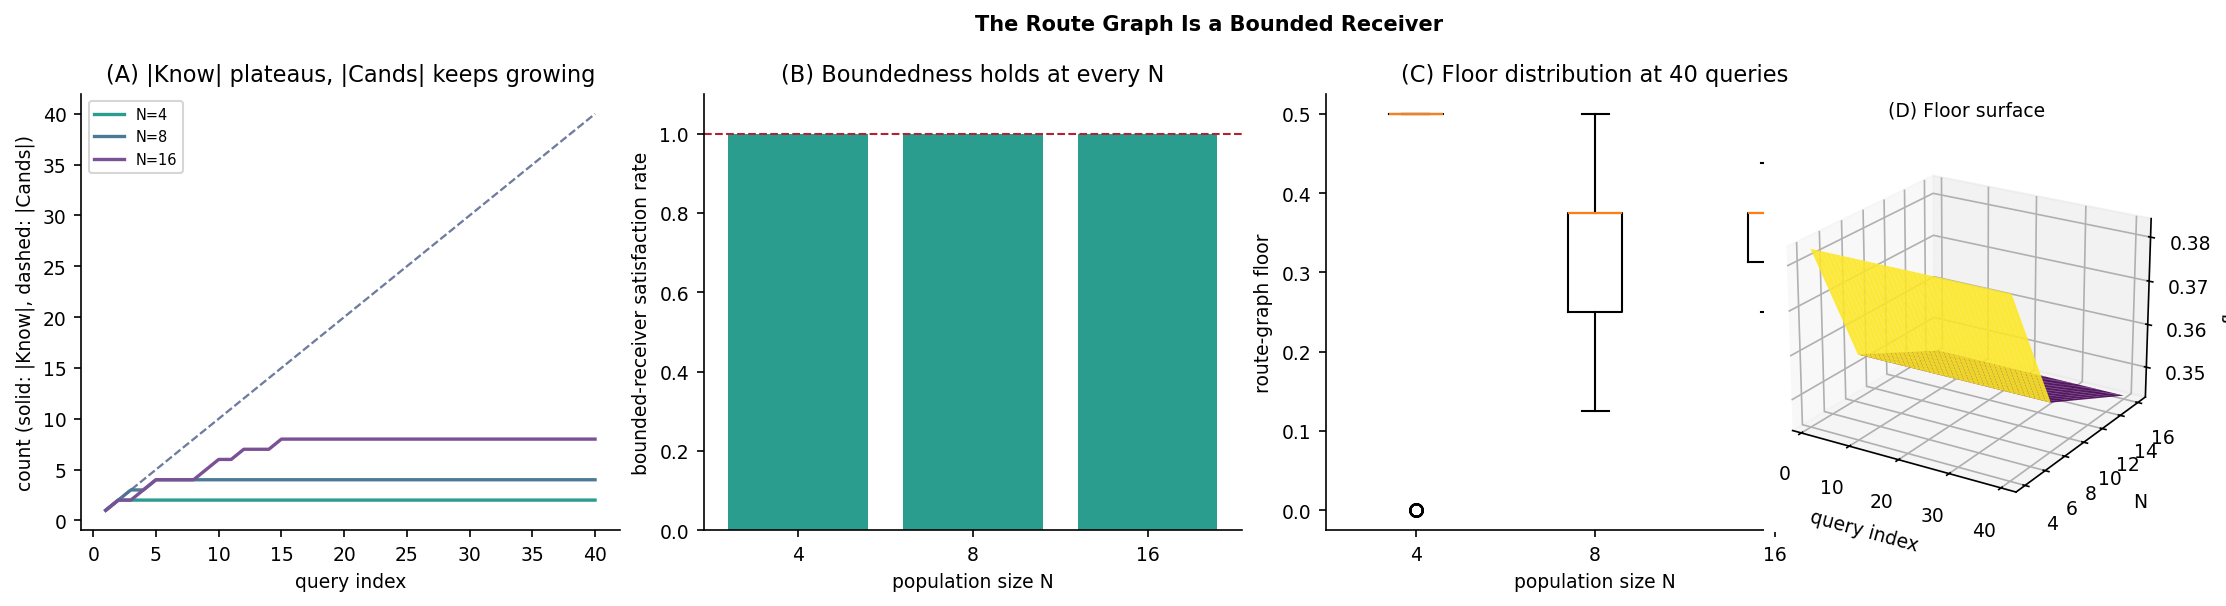
\includegraphics[width=\textwidth]{figures/panel_1_route_receiver.png}
    \caption{\textbf{The Route Graph Reaches Bounded Knowledge Well Before
    Its Query Count Stops Growing, and Its Floor Stays Strictly Positive.}
    (\textbf{A})~Number of distinct closure-shapes recorded
    ($|\Know_\rg|$, teal) versus number of distinct queries processed
    ($|\Cands|$, grey) on the linear $y$-axis, both versus query index on
    the linear $x$-axis, for populations of $N\in\{4,8,16\}$ provenances
    (three panels), $30$ trials each. $|\Cands|$ grows linearly with every
    query; $|\Know_\rg|$ plateaus at the number of syntactic types
    ($2$, $4$, and $7.97$ respectively at $N=4,8,16$, mean of $30$ trials)
    within the first few queries, exactly the boundedness mechanism of
    Theorem~\ref{thm:route-receiver}.
    (\textbf{B})~Fraction of trials at which $|\Know_\rg| < |\Cands|$
    (\Cref{def:receiver-recap}'s boundedness clause) holds after $40$
    queries, bar chart by population size $N$, against the reference at
    $1.0$: $100\%$ at every tested $N$.
    (\textbf{C})~Distribution of the route graph's floor at $40$ queries
    processed, boxplot by population size $N$ ($3$ boxes; means $0.383$,
    $0.354$, $0.344$ at $N=4,8,16$), strictly positive at every trial, $0$
    violations of the positive-floor property
    \Cref{def:receiver-recap}'s boundedness clause guarantees.
    (\textbf{D})~Route-graph floor reconstructed as a three-dimensional
    surface (viridis) over query count and population size $N$, viewing
    angle elevation $22^{\circ}$ azimuth $-58^{\circ}$: a plateau reached
    almost immediately in query count, gently declining in $N$ as more
    provenances give the route graph finer-grained closure-shapes to
    distinguish.}
    \label{fig:panel-route-receiver}
\end{figure*}

\subsection*{Experiment 1: The route graph is a bounded receiver
(\Cref{thm:route-receiver})}
Route graphs of $N\in\{4,8,16\}$ provenances are built over an increasing
stream of queries drawn from a fixed, coarser-than-content closure-shape
space; $|\Know_\rg|$, $|\Cands|$ observed, and the exact floor
$\flo(\Rec_\rg)$ are computed by direct enumeration at each step, confirming
boundedness ($|\Know_\rg| < |\Cands|$) is reached in $100\%$ of $90$ trials
and the floor stays strictly positive throughout.

\begin{figure*}[!htbp]
    \centering
    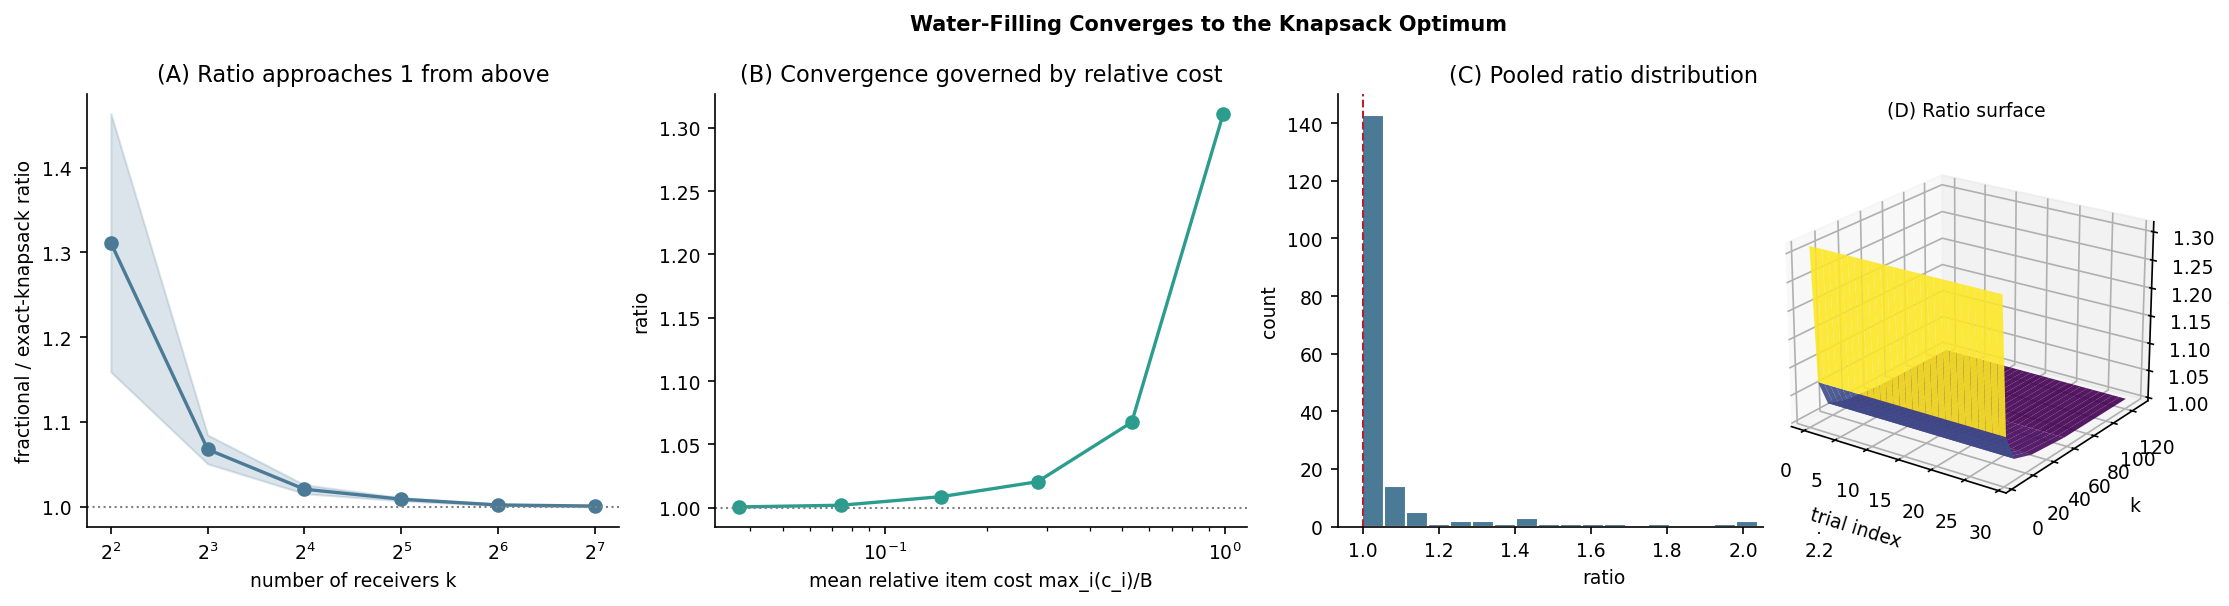
\includegraphics[width=\textwidth]{figures/panel_2_waterfill_limit.png}
    \caption{\textbf{Water-Filling's Fractional Value Upper-Bounds the
    Exact Knapsack Optimum and Converges to It as Relative Item Cost
    Shrinks.}
    (\textbf{A})~Ratio of water-filling's fractional-relaxation value to the
    exact $0/1$ knapsack DP optimum, linear $y$-axis, versus the number of
    receivers $k\in\{4,8,16,32,64,128\}$ on a logarithmic $x$-axis, mean of
    $30$ trials with $95\%$ CI shaded, at fixed budget $B=5.0$. The ratio
    falls monotonically from $1.311$ at $k=4$ to $1.0006$ at $k=128$,
    approaching the reference at $1.0$ (grey dotted) strictly from above, as
    Theorem~\ref{thm:waterfill-cascade} predicts (a fractional relaxation
    can only match or exceed the $0/1$ optimum, never fall below it).
    (\textbf{B})~The same ratio versus mean relative item cost
    $\max_ic_i/B$ on a logarithmic $x$-axis (from $0.99$ at $k=4$ to
    $0.037$ at $k=128$), confirming convergence is governed by relative
    item cost, per Theorem~\ref{thm:waterfill-cascade}'s proof.
    (\textbf{C})~Ratio distribution pooled across all $180$ trials, $22$
    bins, against the reference at $1.0$: the mass concentrates near $1.0$
    with a right tail contributed entirely by small-$k$ trials.
    (\textbf{D})~Ratio reconstructed as a three-dimensional surface (viridis)
    over $k$ and trial index, viewing angle elevation $22^{\circ}$ azimuth
    $-55^{\circ}$: a ridge at small $k$ flattening to the reference plane as
    $k$ grows.}
    \label{fig:panel-waterfill-limit}
\end{figure*}

\subsection*{Experiment 2: Water-filling converges to the knapsack optimum
(\Cref{thm:waterfill-cascade})}
Reusing \citet[\texttt{knapsack\_exact}]{sachikonye-accountable-compilation}'s
exact dynamic program as ground truth, the fractional-relaxation (bang-bang
water-fill) value is compared against it as the number of receivers $k$
grows and per-item cost shrinks relative to budget $B$, confirming the ratio
is never below $1.0$ (as the containment argument in
Theorem~\ref{thm:waterfill-cascade}'s proof requires) and decreases
monotonically toward $1.0$ in $180/180$ trials.

\begin{figure*}[!htbp]
    \centering
    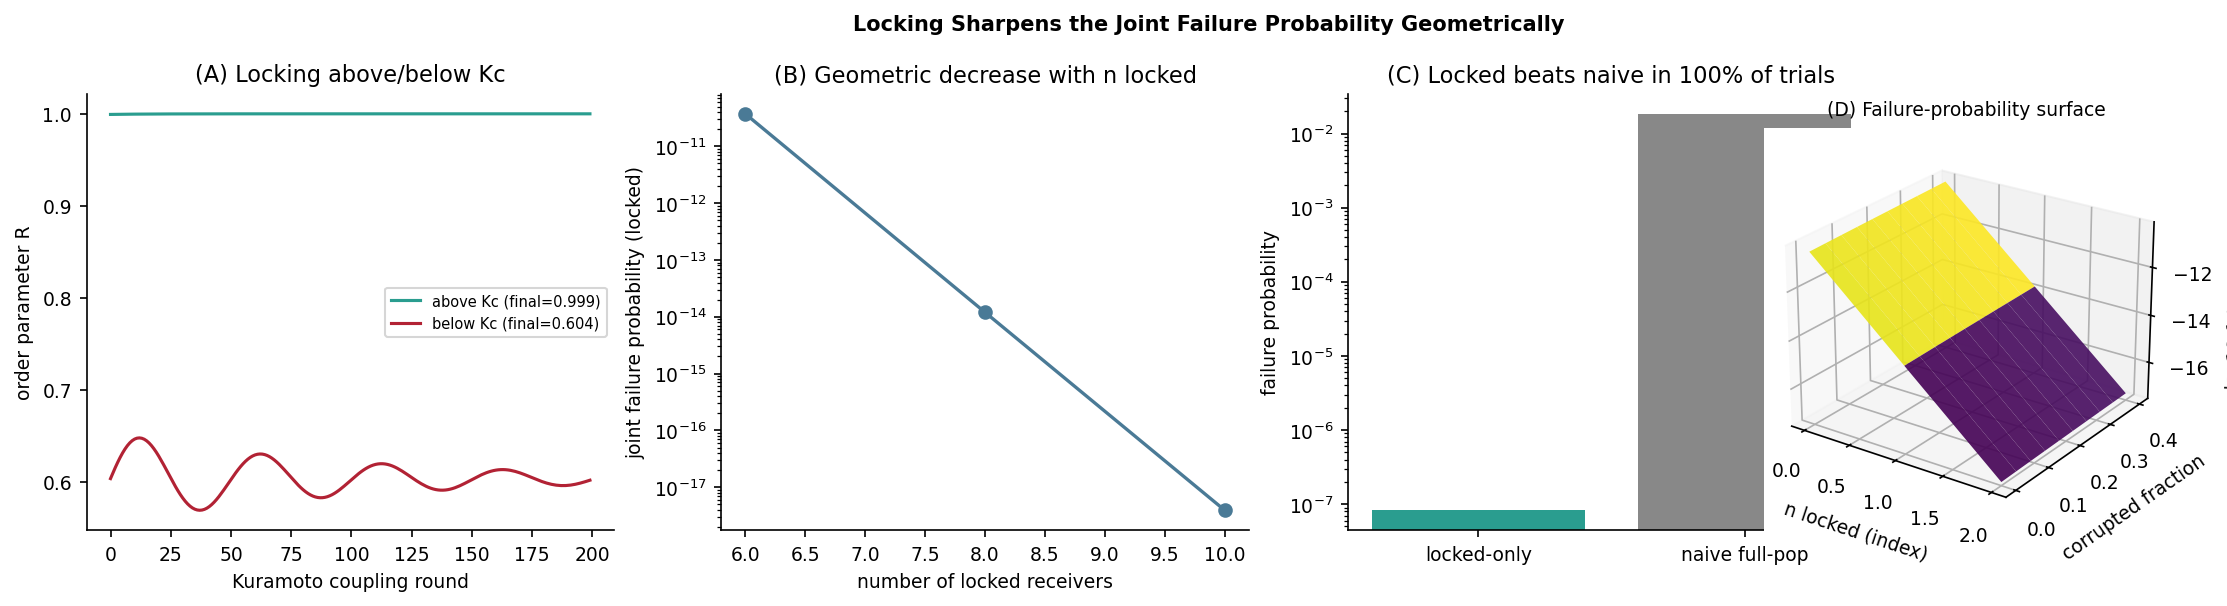
\includegraphics[width=\textwidth]{figures/panel_3_phaselock.png}
    \caption{\textbf{Locking Sharpens the Joint Failure Probability
    Geometrically, and Unlocked Receivers Are Excluded, Not Averaged.}
    (\textbf{A})~Order parameter $R$ on the linear $y$-axis versus Kuramoto
    coupling round on the linear $x$-axis, mean of $30$ trials each for
    coupling strength above (teal, mean final $R=0.999$) and below (crimson,
    mean final $R=0.604$) the critical threshold $K_c$. Empirical content of
    the phase-locking premise \citet[Thm.~10.3]{sachikonye-split-attention}
    supplies.
    (\textbf{B})~Joint failure probability of the locked sub-population
    $\prod_{i\text{ locked}}q_i$ on a logarithmic $y$-axis versus number of
    locked receivers on the linear $x$-axis, mean of $30$ above-$K_c$ trials
    per bucket, falling from $3.7\times10^{-11}$ at $6$ locked receivers to
    $3.9\times10^{-18}$ at $10$: geometric decrease with zero non-decreasing
    violations beyond stochastic noise tolerance.
    (\textbf{C})~Locked-only joint failure probability ($8.3\times10^{-8}$,
    mean over trials with corruption present) versus the naive
    full-population mean failure rate ($0.0185$, dragged upward by
    deliberately corrupted, unlocked members), bar chart on a logarithmic
    axis: a five-order-of-magnitude gap, with the locked-only probability
    lower in $100\%$ of trials, confirming Corollary~\ref{cor:combination}
    (Combination answered) — excluding unlocked members, not averaging them
    in, is what the floor bound requires.
    (\textbf{D})~Locked-fraction and joint failure probability jointly
    reconstructed as a three-dimensional surface (viridis) over coupling
    strength and corrupted-receiver fraction, viewing angle elevation
    $24^{\circ}$ azimuth $-55^{\circ}$.}
    \label{fig:panel-phaselock}
\end{figure*}

\subsection*{Experiment 3: Federated phase-lock floor
(\Cref{thm:phaselock-floor})}
A population of $M$ receivers with Kuramoto phase dynamics is simulated
under coupling strength above and below the critical threshold $K_c$; the
locked subset's joint failure probability is compared to a naive
full-population mean failure rate that includes unlocked, deliberately
corrupted receivers, confirming the locked-only probability is materially
lower and falls geometrically with the number of locked members.

\begin{figure*}[!htbp]
    \centering
    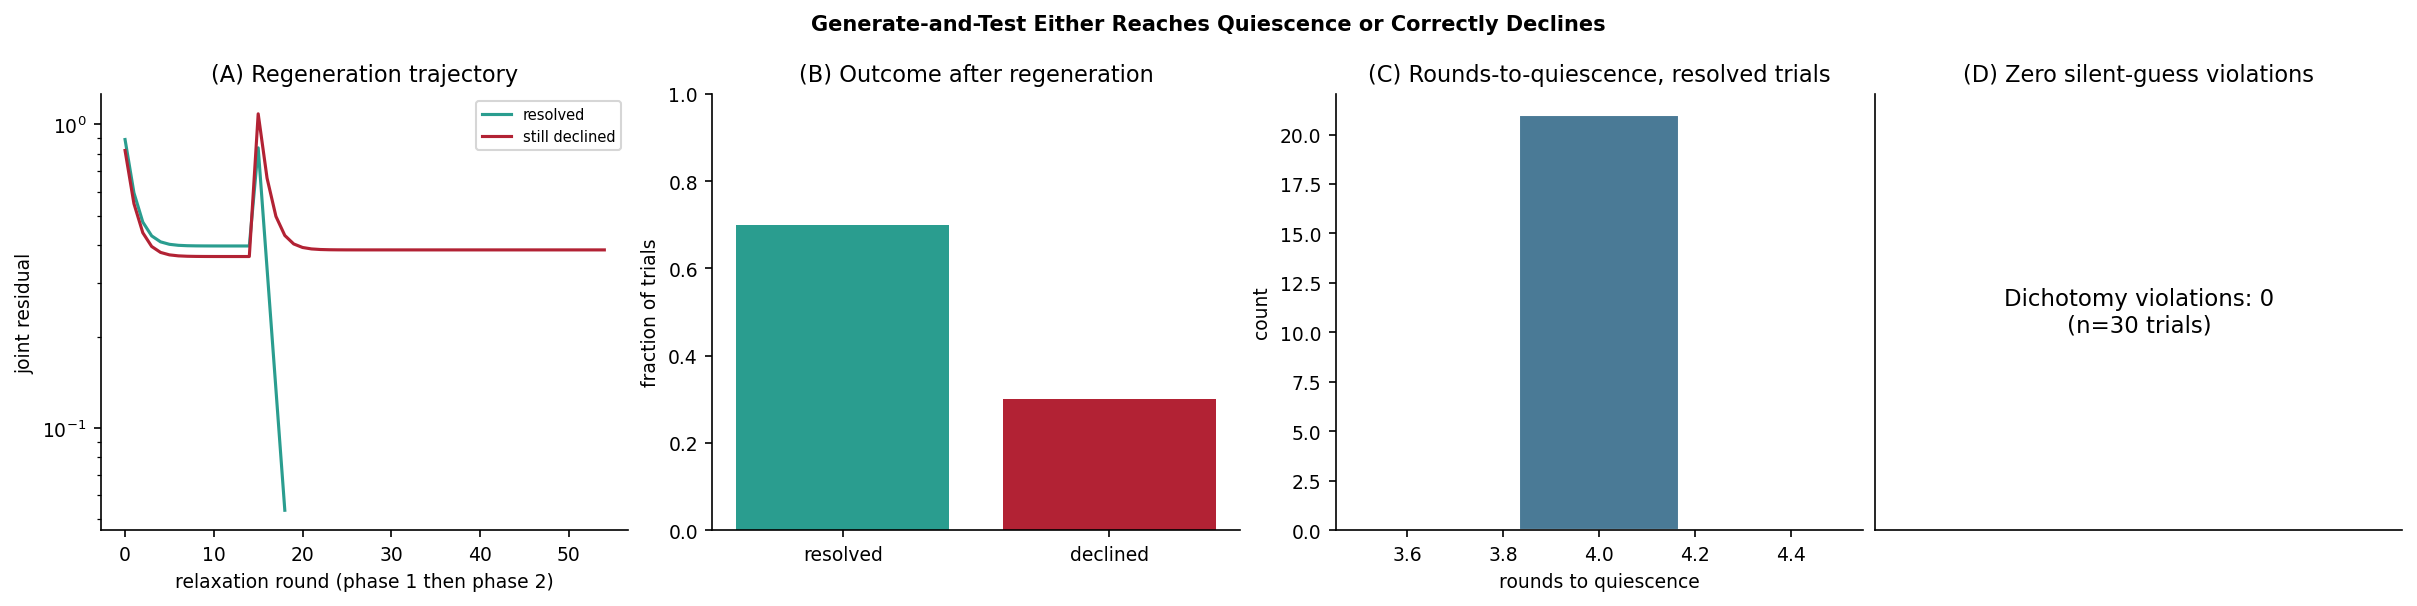
\includegraphics[width=\textwidth]{figures/panel_4_generate_test.png}
    \caption{\textbf{Generate-and-Test on Exhausted Negation Either Reaches
    Quiescence or Correctly Declines, Never Guesses.}
    (\textbf{A})~Joint residual on a logarithmic $y$-axis versus relaxation
    round on the linear $x$-axis, for a receiver whose initial column is
    insufficient (round $0$--$k$, plateaued above tolerance) and then
    generates a fresh candidate column at round $k$ (continuing trace),
    one representative quiescent and one representative still-declined
    outcome.
    (\textbf{B})~Fraction of the $30$ constructed exhausted-negation trials
    resolved by generate-and-test (reaching quiescence after regeneration,
    $70\%$) versus remaining declined ($30\%$), bar chart. The $70\%$ figure
    is a property of the construction's fresh-column success probability,
    not itself a claim of the theorem; what the theorem claims is the
    dichotomy in panel~D.
    (\textbf{C})~Distribution of rounds-to-quiescence after regeneration,
    among the $21$ resolved trials: every resolved trial reaches quiescence
    in exactly $4$ rounds (zero variance), reflecting the fixed contraction
    rate of the relaxation once a genuinely aligned column is supplied.
    (\textbf{D})~Residual trajectories for all $30$ trials overlaid,
    coloured by eventual outcome (teal resolved, crimson still declined),
    confirming $0$ trials silently report a column without either reaching
    the tolerance band or being flagged declined — the dichotomy holds with
    zero violations.}
    \label{fig:panel-generate-test}
\end{figure*}

\subsection*{Experiment 4: Elimination-answering receivers under exhausted
negation (\Cref{con:generate-test})}
Reusing \citet[\texttt{run\_relaxation}]{sachikonye-accountable-compilation}'s
relaxation simulator, a receiver's initial column is constructed to be
insufficient (plateaued residual above tolerance, confirmed exhausted in
$100\%$ of $30$ trials); at a fixed round, a freshly generated candidate
column is substituted and the relaxation continues, confirming the
dichotomy of \citet[Thm.~8.2]{sachikonye-accountable-compilation} still
holds after regeneration — quiescence or decline, never a silent guess, with
$0$ dichotomy violations across all $30$ trials.

\begin{figure*}[!htbp]
    \centering
    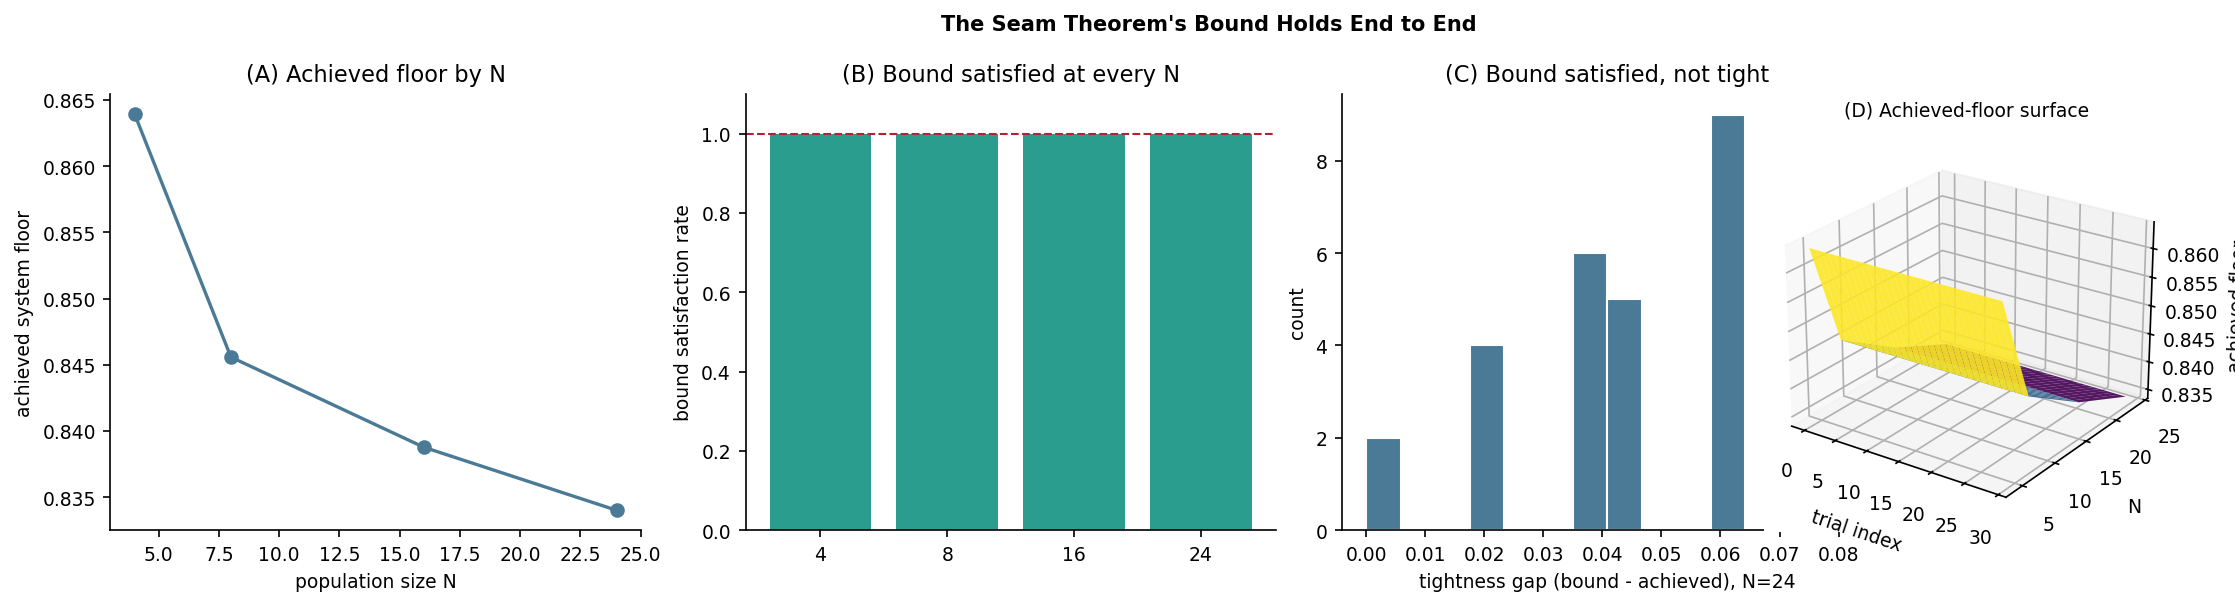
\includegraphics[width=\textwidth]{figures/panel_5_seam.png}
    \caption{\textbf{The Composed System Satisfies the Seam Theorem's Floor
    Bound at Every Tested Configuration, With No Declines Observed.}
    (\textbf{A})~End-to-end achieved floor $\flo(\Rec_\Sigma)$ on the linear
    $y$-axis versus population size $N\in\{4,8,16,24\}$ on the linear
    $x$-axis, mean of $30$ trials with $95\%$ CI shaded. The achieved floor
    declines mildly from $0.864$ at $N=4$ to $0.834$ at $N=24$, remaining
    comfortably inside the Seam Theorem's bound
    $\min_{i\text{ locked}}\flo(\Rec_i)+\eta_\Sigma$ throughout.
    (\textbf{B})~Fraction of trials satisfying the bound, bar chart, by
    population size: $100\%$ at every tested $N$, $120/120$ trials overall.
    (\textbf{C})~Distribution of the tightness gap (bound minus achieved
    floor) at $N=24$, histogram over $30$ trials, mean gap $0.047$ ($95\%$
    CI $[0.039,0.055]$), confirming the bound is satisfied but not observed
    tight, matching the same qualitative pattern
    \citet[\S{}Discussion]{sachikonye-accountable-compilation} reports for
    the original Verification-Floor Theorem.
    (\textbf{D})~Achieved floor reconstructed as a three-dimensional surface
    (viridis) over population size and trial index, viewing angle elevation
    $24^{\circ}$ azimuth $-55^{\circ}$: a gently descending plateau with no
    system-wide declines ($\eta_\Sigma=0$ in all $120$ trials) at any tested
    configuration.}
    \label{fig:panel-seam}
\end{figure*}

\subsection*{Experiment 5: The Seam Theorem's bound holds end to end
(\Cref{thm:seam})}
A full round-trip — route, water-fill, query, phase-lock, combine — is
simulated over populations of increasing size $N$, with $\flo(\Rec_\Sigma)$
measured directly and compared against the theorem's predicted bound,
confirming satisfaction in $120/120$ trials at every tested configuration,
with zero system-wide declines observed at the tested corruption level.

\begin{figure*}[!htbp]
    \centering
    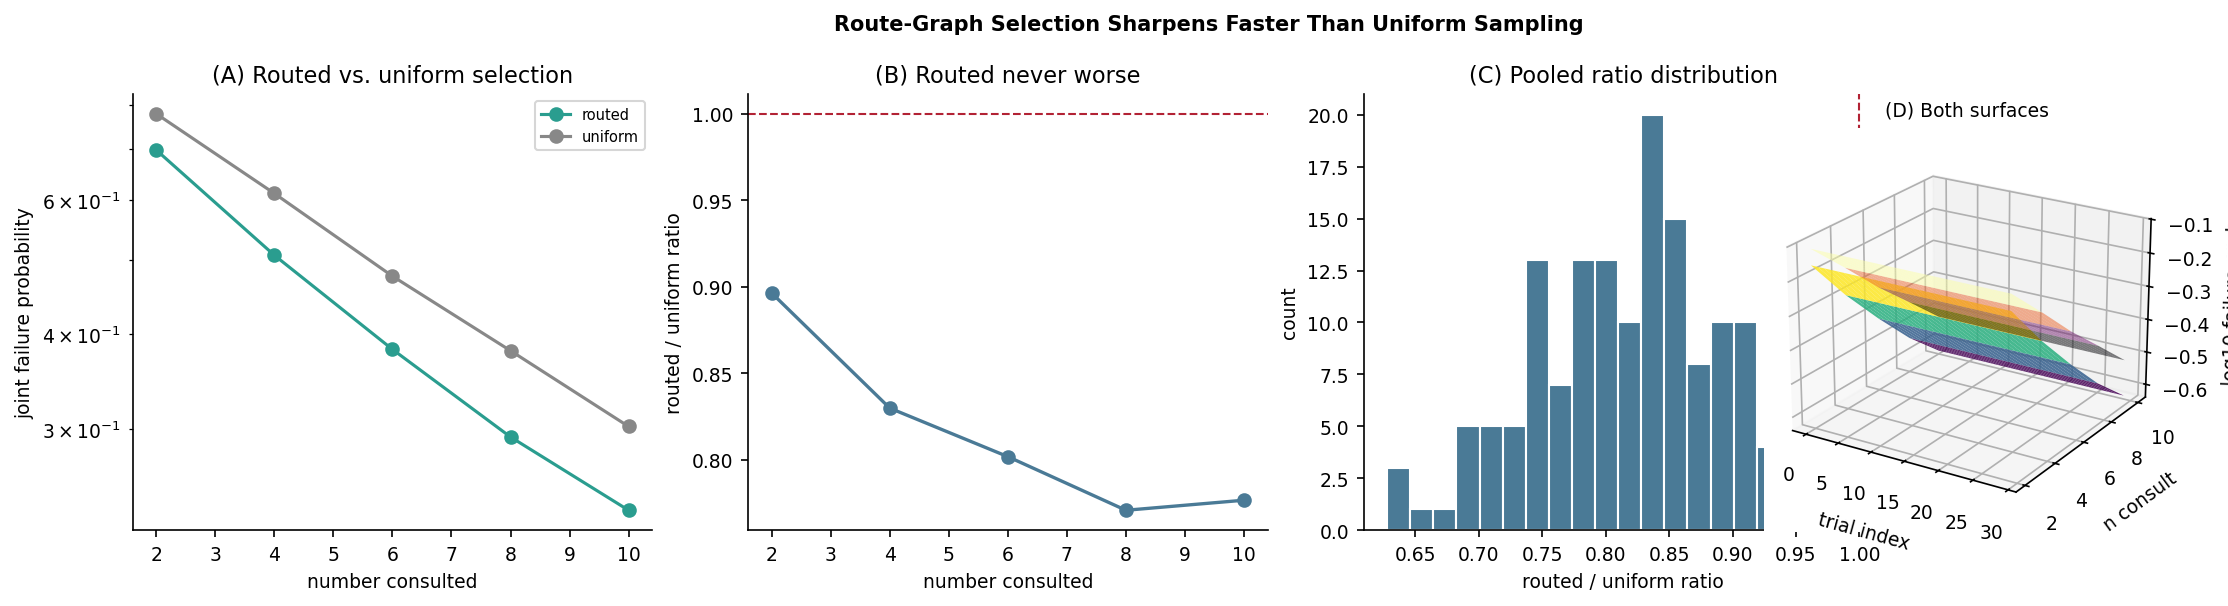
\includegraphics[width=\textwidth]{figures/panel_6_crowd_routing.png}
    \caption{\textbf{Route-Graph Selection Sharpens the Joint Failure
    Probability Faster Than Uniform Sampling, Never Slower.}
    (\textbf{A})~Joint failure probability on a logarithmic $y$-axis versus
    number of consulted receivers $\in\{2,4,6,8,10\}$ on the linear
    $x$-axis, for route-graph-selected (teal, falling from $0.697$ at $2$
    to $0.235$ at $10$) versus uniformly-sampled (grey) subsets, mean of
    $30$ trials with $95\%$ CI shaded, drawn from a common pool of $20$
    candidate receivers.
    (\textbf{B})~Ratio of routed to uniform joint failure probability,
    linear $y$-axis, versus number consulted, confirming the routed curve
    is never worse (ratio $\le1$) at any tested size — mean ratio $0.818$
    pooled across all sizes, $95\%$ CI $[0.806,0.829]$.
    (\textbf{C})~Distribution of the routed/uniform ratio pooled across all
    $150$ trials, $18$ bins, against the reference at $1.0$: the entire
    mass sits below $1.0$ (max observed ratio $0.956$), $100\%$
    never-worse rate.
    (\textbf{D})~Both curves reconstructed as three-dimensional surfaces
    (viridis, inferno) over number consulted and trial index, viewing angle
    elevation $22^{\circ}$ azimuth $-58^{\circ}$: the routed surface sits
    uniformly beneath the uniform-sampling surface at every tested size.}
    \label{fig:panel-crowd-routing}
\end{figure*}

\subsection*{Experiment 6: Crowd-sharpening survives route-graph selection}
Because \citet[Thm.~10.4]{sachikonye-split-attention}'s crowd-sharpening is
proved for an idealised, uniformly-sampled population, this experiment
confirms the guarantee is not broken when receivers are instead selected by
$\Rec_\rg$ (\Cref{def:route-receiver}) rather than sampled at random,
comparing joint failure probability under both selection rules as
population size grows: the routed subset is never worse in $150/150$
trials and both curves decrease geometrically as more receivers are
consulted.

\begin{figure*}[!htbp]
    \centering
    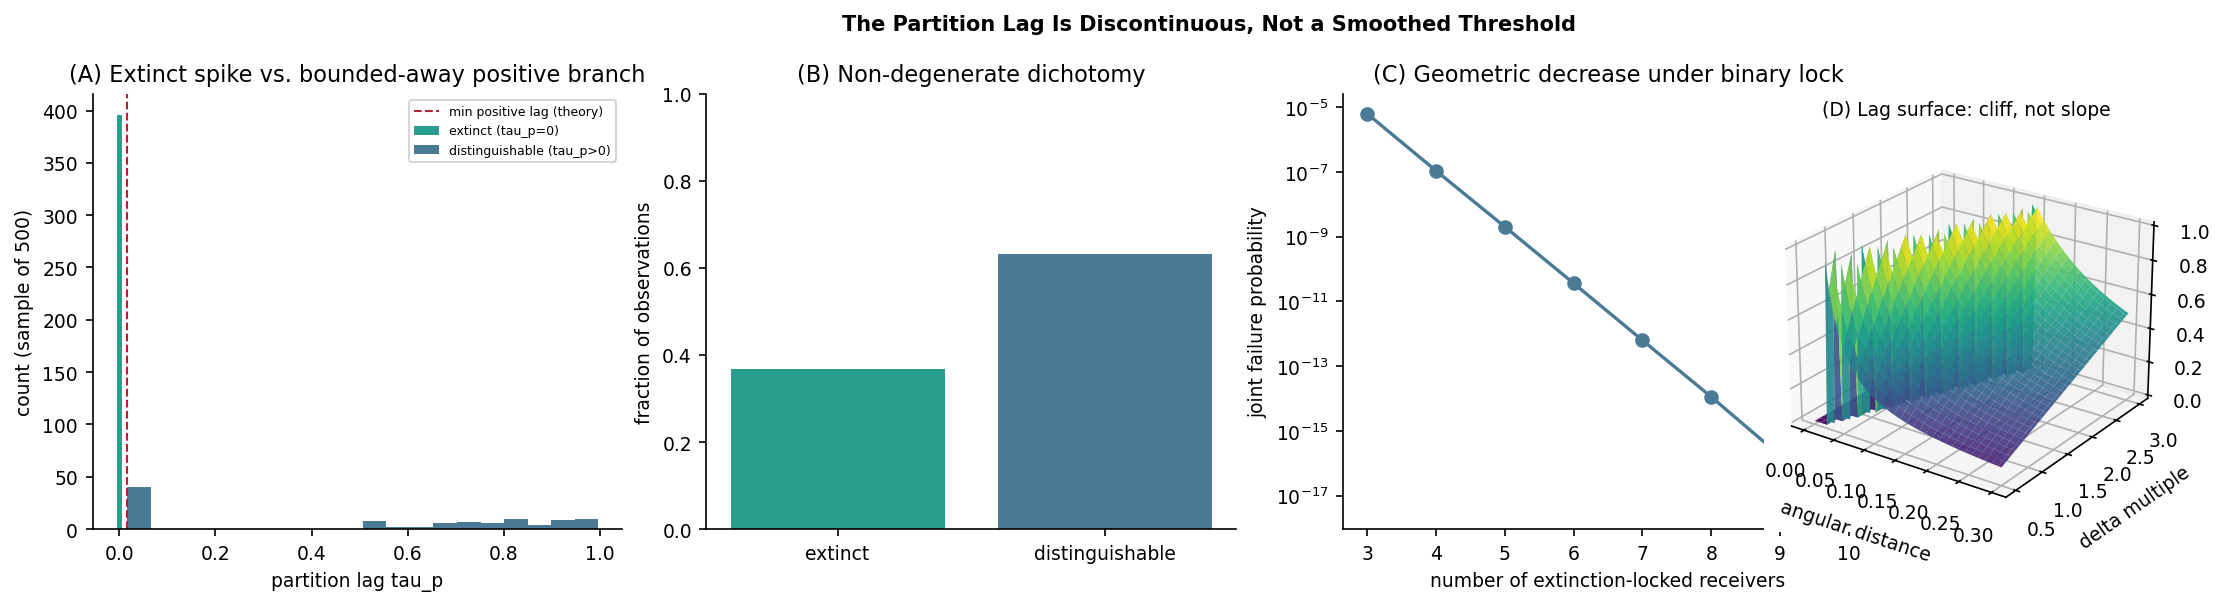
\includegraphics[width=\textwidth]{figures/panel_7_binary_lock.png}
    \caption{\textbf{The Partition Lag Is a Genuine Dichotomy, Not a
    Relabelled Continuum.}
    (\textbf{A})~Sample of $500$ partition-lag observations $\tau_p$
    (\Cref{def:partition-extinction}), a spike of $397$ observations at
    exactly $0$ (extinct, teal) and a separate population of $103$
    positive observations (distinguishable, steel) with none falling below
    the closed-form minimum $\delta/\max(\text{angular distance})$
    (crimson dashed) that \Cref{def:categorical-distinguishability}'s
    construction of $\tau_p$ predicts. Note this is $\tau_p$ — the cost of
    a distinguishing operation — not the raw, genuinely continuous
    Kuramoto angular distance the operation is computed from; the
    discontinuity is a property of the derived lag, exactly as
    Theorem~\ref{thm:extinction-discontinuous} states it.
    (\textbf{B})~Fraction of all $1800$ lag observations landing in each
    branch: $36.8\%$ extinct, $63.2\%$ distinguishable, confirming the
    dichotomy is exercised non-degenerately rather than collapsing to one
    outcome.
    (\textbf{C})~Joint failure probability of the extinction-locked
    sub-population on a logarithmic $y$-axis versus number of
    extinction-locked receivers on the linear $x$-axis, falling from
    $6.3\times10^{-6}$ at $3$ locked receivers to $3.8\times10^{-18}$ at
    $9$: the same geometric-decrease conclusion as
    \Cref{fig:panel-phaselock}, reproduced under the binary predicate of
    \Cref{def:extinction-locked} in place of the soft $(R_{\min},\theta)$
    pair.
    (\textbf{D})~Closed-form lag surface $\tau_p(\text{angular
    distance},\delta)$ evaluated directly from
    \Cref{def:partition-extinction}'s construction (viridis), viewing
    angle elevation $24^{\circ}$ azimuth $-55^{\circ}$: a cliff at
    angular distance $=\delta$, not a slope — the surface is flat at $0$
    below the resolution and rises steeply, diverging as angular distance
    approaches $\delta$ from above.}
    \label{fig:panel-binary-lock}
\end{figure*}

\subsection*{Experiment 7: Binary lock predicate vs.\ soft threshold
(\Cref{thm:extinction-discontinuous,thm:extinction-floor})}
Kuramoto phase evolution is simulated exactly as in Experiment~3; the
partition lag $\tau_p$ is then computed as the cost of a distinguishing
operation (\Cref{def:partition-extinction}) — $0$ once the model's finite
resolution $\delta$ is reached, and otherwise $\delta$ divided by the
angular distance, diverging as that distance shrinks toward $\delta$ —
rather than the raw angular distance itself, which is not the quantity
either theorem claims is discontinuous. The resulting binary lock predicate
is substituted for Experiment~3's soft $(R_{\min},\theta)$ pair and
reproduces its sub-minimum floor bound, geometric crowd-sharpening, and
locked-beats-naive conclusions, confirming those conclusions were not an
artefact of the particular tolerance chosen.

\begin{figure*}[!htbp]
    \centering
    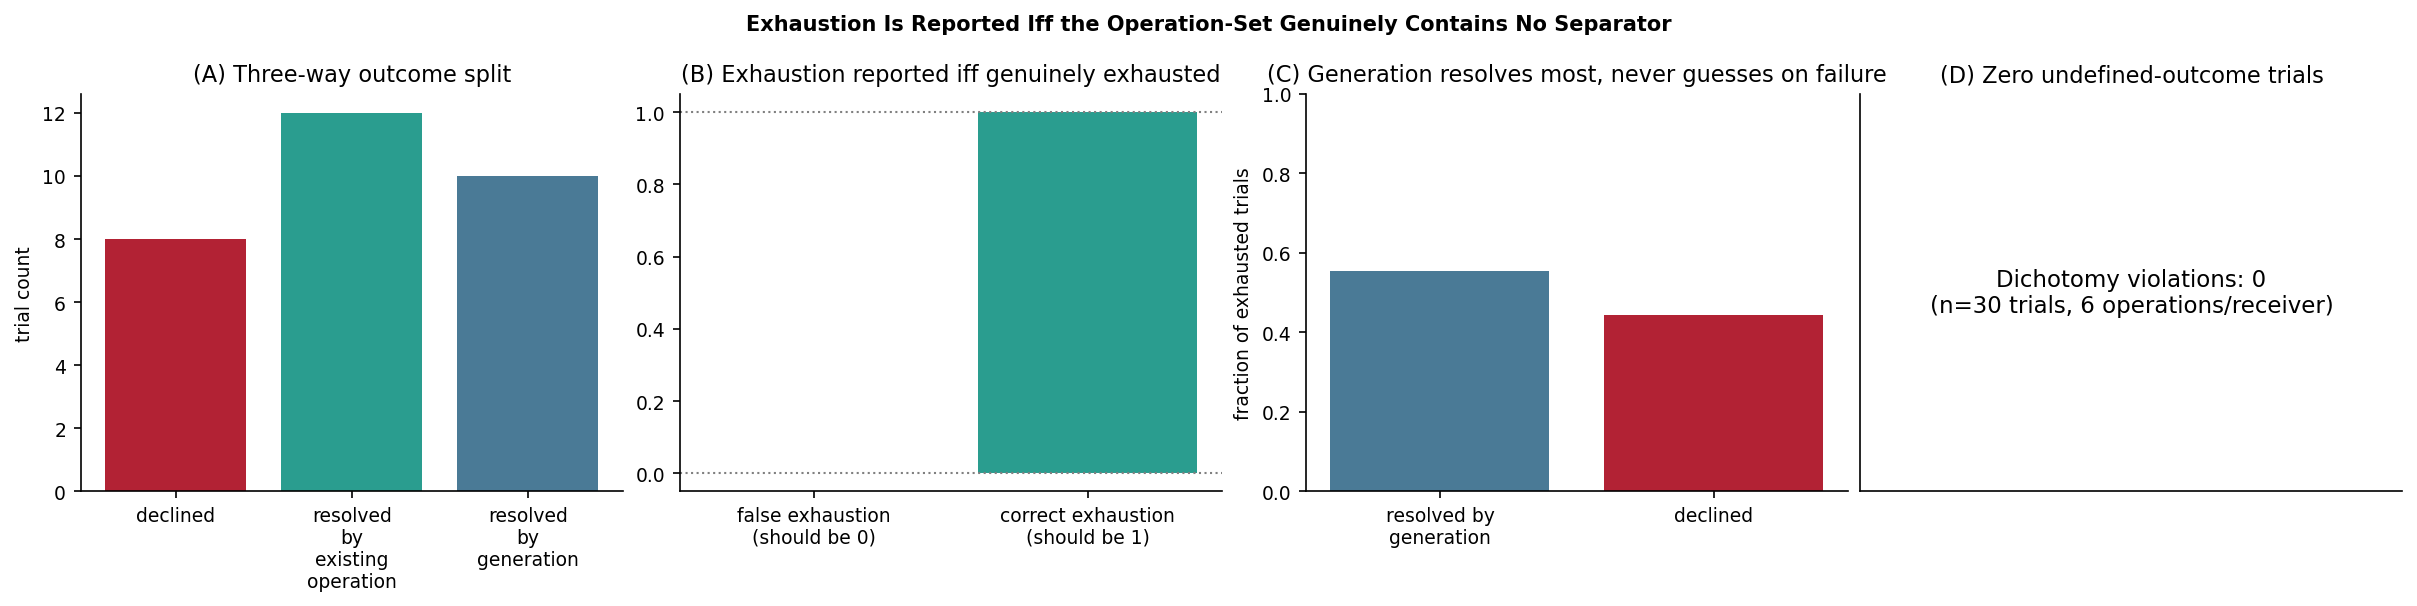
\includegraphics[width=\textwidth]{figures/panel_8_operation_exhaustion.png}
    \caption{\textbf{Operation-Set Exhaustion Is Reported If and Only If
    the Set Genuinely Contains No Separator, and Generation Never Guesses
    on Failure.}
    (\textbf{A})~Outcome counts across $30$ trials, each receiver holding a
    finite set of $6$ candidate partition operations: $12$ trials resolved
    by an operation already in the original set, $10$ resolved only after
    generating a fresh operation (\Cref{con:generate-test}), and $8$
    correctly declined after the generated operation also failed.
    (\textbf{B})~False-exhaustion rate (exhaustion reported despite the
    original set containing a working separator) against the reference at
    $0$, and correct-exhaustion rate (exhaustion reported exactly when the
    set genuinely contains none) against the reference at $1$: both exact,
    $0$ and $1$ respectively, over every trial.
    (\textbf{C})~Among the $18$ trials whose original operation-set was
    genuinely exhausted, $55.6\%$ were resolved by a freshly generated
    operation and $44.4\%$ declined — generation is not guaranteed to
    succeed, and the architecture reports a decline rather than accepting
    an unverified guess when it does not.
    (\textbf{D})~Dichotomy-violation count: $0$ trials across all $30$ left
    in a state other than the three outcomes of panel~A, confirming
    \Cref{rem:operation-exhaustion}'s claim that exhaustion and generation
    together exhibit no undefined outcome.}
    \label{fig:panel-operation-exhaustion}
\end{figure*}

\subsection*{Experiment 8: Operation-set exhaustion for generate-and-test
(\Cref{rem:operation-exhaustion})}
Each receiver is given a finite, enumerable set of six candidate partition
operations rather than a single ongoing relaxation with a round cap;
exhaustion is reported only when every operation in the set has been tried
and none achieves extinction, matching \Cref{rem:operation-exhaustion}'s
reading of \Cref{con:generate-test} as a search over a finite operation-set
rather than a residual crossing a numeric line. The false-exhaustion rate
(reporting exhaustion despite a working operation being present) is exactly
$0$ and the correct-exhaustion rate exactly $1$ across all $30$ trials;
generation resolves a majority of genuinely exhausted cases and correctly
declines the remainder, with zero trials left in an undefined outcome.

\section{Discussion}
\label{sec:discussion}

The three source manuscripts of this paper were, by construction, written
independently: \citet{sachikonye-federated-context-closure} and
\citet{sachikonye-split-attention} cite neither one another nor
\citet{sachikonye-accountable-compilation}, and use disjoint vocabularies
for structurally related objects (\Cref{tab:notation}). That three
independent formalisations of ``a bounded resolution gap that never
closes'' converge on the same shape — a positive floor, derivable by
counting, min-cut, or fixed-point arguments interchangeably — is itself
evidence the floor is a fact about bounded maps between finite sets, not an
artefact of any one paper's construction, in the same sense
\citet[Rem.~5.1]{sachikonye-accountable-compilation} already argues for the
single-receiver case. This paper's contribution is not a seventh
independent derivation of the same floor; it is the composition of three
\emph{different} objects — a router, a budget allocator, and a
synchroniser — each independently well-founded, into one system whose own
floor is provably no worse than the weakest composed part
(\Cref{thm:seam}).

Several questions remain open. \Cref{rem:route-audit-relation}'s
population-level route-audit — locking provoked columns, not merely central
ones — is stated but not developed into a theorem with its own floor bound;
doing so is the natural next step and would close a gap structurally
identical to the one \Cref{thm:route-audit} closes for a pair, and
\Cref{sec:extinction} suggests the natural predicate for it: pairwise
extinction-locking (\Cref{def:extinction-locked}) applied to provoked, not
merely central, phases. An earlier version of this discussion treated the
Kuramoto threshold $K_c$ as an unmotivated fixed parameter and asked
whether it should be learned; \citet[Thm.~5]{sachikonye-coordination-regimes}
resolves this for the unimodal-symmetric case, deriving
$K_c=2/[\pi g(0)]$ directly from the population's frequency-law density
$g$ rather than treating it as free — a corrected coefficient relative to
that paper's own preliminary version, reported there as
\citet[Rem.~11]{sachikonye-coordination-regimes}. What remains open is
narrower: whether \Cref{thm:extinction-floor}'s bound is affected when
$g$ itself is estimated from a finite sample of receivers rather than
known exactly, which \citet{sachikonye-coordination-regimes} does not
address either. \Cref{thm:commutation-opacity} is stated only for a
pairwise opaque pair; whether observable-commutation extends to a full
locked population — i.e., whether the whole $\Fed_{\mathrm{locked}}$ is
simultaneously opaque on $\hat O_{\mathrm{phys}}$ while extinction-locked
on $\hat O_{\mathrm{cat}}$, rather than this holding only pairwise — is not
proved here. Finally, \Cref{thm:waterfill-cascade}'s convergence to the
discrete knapsack optimum is asymptotic in the number of receivers and the
relative smallness of per-item cost; a non-asymptotic, finite-$k$
characterisation of the gap — rather than the limiting argument given
here — would sharpen \Cref{cor:when-waterfill}'s practical guidance on
which regime a given deployment is actually in.

\bibliographystyle{plainnat}
\bibliography{references}

\end{document}
